\documentclass[12pt]{article}
%\usepackage{paper} %if the document does not compile properly for you on the initial build, uncomment \usepackage{paper} and build again. This should force MikTeX to install package "paper"
\usepackage[margin=1in]{geometry}
\usepackage{float}
\usepackage{natbib}
\bibliographystyle{apsr}
\usepackage{graphicx}
\graphicspath{ {../fig/} }
\usepackage{setspace}
\setstretch{2}
\usepackage[super]{nth}
\usepackage{booktabs}
\usepackage{makecell}
\usepackage{amsmath}
\usepackage{dcolumn}
%\usepackage{authblk}
\usepackage{hyperref}
%\usepackage{etoolbox}
%\AtBeginEnvironment{quote}{\singlespacing\small}

\begin{document}

\title{First Year Paper:\\ \large{\citet{iyengar2012affect}}}
\author{Robert Lytle}
\date{\today}
\maketitle
\thispagestyle{empty}
\clearpage
\section{Introduction}
The question ``Has the mass public polarized alongside elites?" has been the subject of an enormous amount of scholarly debate. This debate has been held largely in terms of ideology, with scholars leveraging competing evidence showing \citep{abramowitz2010disappearing} or not showing \citep{fiorina2012disconnect} mass-level polarization. \cite{iyengar2012affect} argue that affect (one's emotional valence towards a stimulus) rather than ideology should be used to evaluate levels of mass polarization. 

While the authors leverage a variety of publicly available observational datasets to demonstrate that Democrats and Republicans exhibit increasing animosity towards out-partisans in this paper, I replicate the findings of \cite{iyengar2012affect} as they relate to the effect of policy preferences and party identification on affective polarization, and extend the original work first by applying the authors models to more recent 2016 data alongside the replication and then by respecifying the models to a more appropriate functional form.


\section{Summary of \cite{iyengar2012affect}}
\textit{Affect, Not Ideology} is an ambitious work; seeking to describe the historical trends of affective polarization and to establish a causal chain between hostile media, party-ID, and mass-level affective polarization. This analysis is done in service of the authors' central argument: that Americanist scholars of polarization should study the attitudes of voters towards members of the out-party, not just the ideological differences between opposing parties.

The vast majority of scholars have evaluated polarization in terms of divergent policy preferences between parties and their supporters and have produced contradictory results. While virtually all agree that \textit{elites} have become more polarized, some argue this elite polarization is in response to an increasingly polarized \textit{public} \citep{abramowitz2010disappearing} and some argue against the notion of mass polarization altogether \citep{fiorina2012disconnect, fiorina2005culture}. Still other scholars have argued that observed polarization is not the result of increasingly extreme policy positions on the part of Democrats and Republicans, but the result of previously ideologically heterodox partisans sorting themselves into more appropriate parties \citep{levendusky2009partisan}.

Each of the works discussed in the previous paragraph share a common focus on partisans' \textit{ideology}. Iyengar, Sood, and Lelkes identify this commonality and argue that, since most people have a limited conception of their own ideology \citep{converse1964nature}, and tend to have conflicting \citep{mcclosky1984american} and ideologically incoherent views \citep[p. 76--96]{zaller1992nature}, ideological differences are not a suitable metric by which to gauge mass polarization. In the view of the authors, partisans' affect towards their opponents is a more consistent and substantively meaningful diagnostic of the degree of mass polarization.

To demonstrate this, the authors leverage several existing survey datasets and an advertising dataset\footnote{\textit{ANES Cumulative Study, YouGov/Polimetrix 2008 Election Study}, a \textit{YouGov 2011 multi-national study, Almond \& Verba (1960), Blair Center Election Study}, an \textit{AP Yahoo! News 2008} Election Study and the \textit{Wisconsin Advertising Project}. The implications for validity in using survey data will be discussed in greater detail in section 3.}. The survey data are used first to describe the degree of affective polarization, and are then used in conjunction with the advertisement data to establish a causal link between exposure to hostile political media and affective polarization. Survey data from the United Kingdom is included in the descriptive portion of the research, intended by the authors to serve as a pseudo-control for country-level effects \citep[p. 407]{iyengar2012affect}, comparing a country with parties whose ideology is more salient (the U.K.) to the U.S.

In a series of regression analyses presented in the table below, the authors use data from the ANES to argue that cultural attitudes have no effect on affective polarization, while economic attitudes are only loosely related. Rather, they argue, the simple strength of one's partisan identification explains the degree to which they feel warmly towards their in-party and coldly towards the outparty. The dependent variable in these analyses is ``net partisan affect" (NPA), the difference between a respondent's in-party and out-party feeling thermometers used to measure the degree to which a survey respondent feels warmly or coldly towards another group. My principal focus in this paper will be to replicate these results, extending the data to 2016 before critiquing and respecifying the model.

\begin{figure}[H]
\center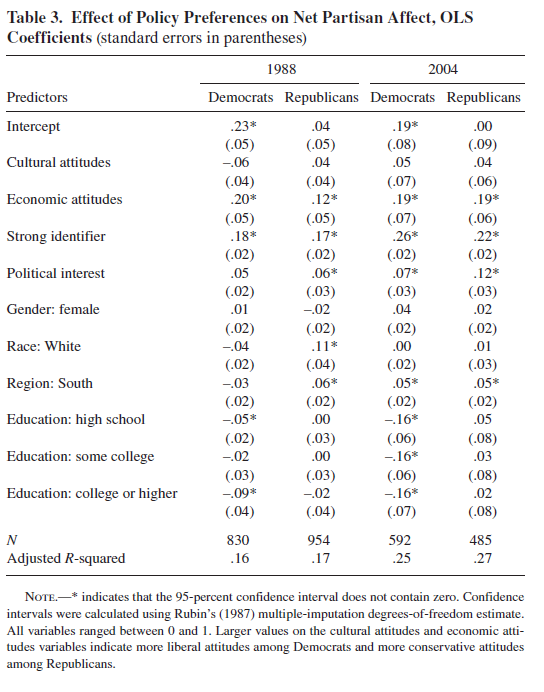
\includegraphics[width=5in]{isl-fig-3.png}
\caption{\label{fig:cdf-avg}\textit{\textbf{The original results from Iyengar, Sood, and Lelkes (2012).} These results are the primary focus of this paper, and will be referenced throughout this piece.}}
\end{figure}

In short: \citeauthor{iyengar2012affect} identify a shortcoming in the ongoing debate over the existence of mass-level polarization---that scholars have focused exclusively on partisans' ideology. Instead, they argue that analyses of ideology are insufficient means by which to evaluate mass polarization. The authors argue for a new conception of division: partisans' affect towards their opponents. Iyengar et al. show that partisans are becoming increasingly divided from (and hostile towards) one another and posit that this division is the result of increasingly hostile media, rather than ideological differences between partisans. Therefore, ideological homogeneity between Democrats and Republicans is not sufficient evidence of a broader lack of polarization. 
\section{Replication}

\subsection{Role of Ideology in Affective Polarization}

Ideology, the authors contend, plays a minimal role in driving out-party animus. This conclusion is reached through the application of a Two-Factor Structural Equation Model in which both respondents' cultural positions (gay rights, women's place, and abortion) and their economic positions (social security, healthcare, jobs, essential services) are allowed to affect one of three dependent feeling thermometer variables: in-party, out-party, and the difference of the two. Also included in the regression model are several covariates indicating political interest, whether a respondent is a strong partisan, gender, region (whether a respondent is a southerner), and education. While my replication forgoes the structural equation model used by the authors, both the author's model and my replication us an OLS model of the form:

\begin{equation}
\begin{split}
\hat{\mathit{Net Partisan Affect}} = \alpha + \hat{\beta}_1{\mathit{Culture}} + \hat{\beta}_2\mathit{Econ} + \hat{\gamma}_3\mathit{Strong Partisan} +  \hat{\beta}_4\mathit{Interest} +  \gamma_5\mathit{Female} + \\ \hat{\gamma}_6\mathit{South} + \hat{\gamma}_7\mathit{High School} + \hat{\gamma}_8\mathit{Some College} + \hat{\gamma}_9\mathit{Adv. Deg}
\end{split}
\end{equation}

\noindent where dummy variables are indicated by a gamma coefficient, to similar results, as shown in section 3.4.

\subsection{Survey Validity Issues}

Surveys are notoriously vulnerable to issues of framing, priming, and response instability \citep[p. 53--75]{zaller1992nature}, which at best introduce noise in the data and at worst (or at the most interesting, depending on one's perspective) are illustrative of a broader problem with the measurement of public opinion---that many people are simply ``Making it up as [they] go along", to borrow a phrase from Zaller. While these problems are not addressed by \citeauthor{iyengar2012affect} \textit{post facto}; surveys (including the ANES, from which much of these data are drawn) take steps to ameliorate some of the threat from other forms of response bias, often randomizing the order in which questions are asked so as to avoid priming respondents. Still, the larger problem of instability is a more fundamental problem, and one that is not addressed in the text.

A third validity concern of these data is the possibility that respondents have under reported their attachment to their party. As people generally express a preference for bipartisanship \citep{harbridge2014public}, there is logical reason to believe respondents' desire to appear less partisan could lead to Hawthorne effects or social-desirability bias, posing a potential threat to the construct validity of the findings \citep[p. 73, Table 3.1 Item 8]{shadish2002experimental}. Fortunately, if the results are the product of social desirability bias they should \textit{underestimate} the degree of affective polarization. Thus the possibility of unaccounted for social desirability bias does not pose a major threat to the core findings of the paper.


\subsection{Execution \& Results}

On the next page, I present the results of the replication of Iyengar, Sood, and Lelkes' original models. I estimate six models of the effect of covariates on net partisan affect. The first four models replicate Table 3 of \cite{iyengar2012affect} (fig. 1 of this paper), while models five and six apply the regression to both Democrats and Republicans in 2016. Aside from subsetting on party ID and year, the specification of each model is identical. All six are linear, OLS regressions.

Data for this extension are taken from the ANES cumulative data file, which has been asking respondents to report a partisan feeling thermometer since 1978. Rscripts from \citeauthor{iyengar2012affect}'s original paper were supplied by Gaurav Sood, to ensure that the variables used in my replication were the same used in the original piece. The bulk of the code used to wrangle the ANES data and conducted replication was written by myself in RStudio, making heavy use of the \texttt{tidyverse} and \texttt{stargazer} packages, as well as Gaurav Sood's own \texttt{goji} package \footnote{https://github.com/soodoku/goji}.

Gender, Region, Race, and the education categories are each dummy variables included as Demographic controls. ``Strong Partisan" is a dummy variable indicating that a respondent identifies as strongly Democratic or Republican, and ``Political Knowledge" is an interviewer's assessment of the respondent's general political knowledge, averaged across a record made at the beginning and end of their interview on a five point scale. It has been coded so that high values indicate high levels of political knowledge.

For convenience, each variable has been rescaled to a range [0,1], as in the original paper. In other words, the coefficients presented in the table bellow indicate the change in Net Partisan Affect when moving from the lowest to highest possible value of each variable. The cultural and economic attitude items are both constructed from a variety of ANES questions which present respondents with an issue (such as whether social security should be expanded) and ask them to place their ideal point on a scale ranging from most to least conservative. These items were rescaled such that high values represented the ideological position most consistent with their party ID (e.g., a ``1" would be a perfectly liberal response for a Democrat and a perfectly conservative response for a Republican). These responses were then averaged across the relevant issue areas.

This method of variable construction is likely problematic---it is not clear that these responses are truly quantitative. Even if responses to the same question are quantitative, it is not unlikely that a respondent views the statements ``Social Security should be expanded", and ``The government should provide health insurance" as being mathematically equivalent in terms of their ideological liberalism, but the measure used in this replication assumes so nonetheless.

This potentially dubious coding decision was made to replicate as closely as possible the measures used by Iyengar, Sood, and Lelkes, who use a structural equation model to estimate the effects of economic and cultural attitudes on NPA. The authors' results are generally robust to my simplified model, the magnitude of effects observed varying only slightly. The core claims made by the authors; that strong partisan identification and to a lesser extent, economic attitudes, are driving polarization hold, with (minor) variation in the effects of demographic controls.

% Table created by stargazer v.5.2.2 by Marek Hlavac, Harvard University. E-mail: hlavac at fas.harvard.edu
% Date and time: Tue, Apr 21, 2020 - 3:25:31 AM
% Requires LaTeX packages: dcolumn 
\begin{table}[H] \centering 
  \caption{Original Models (Extended to 2016)} 
  \label{} 
\begin{tabular}{@{\extracolsep{-10pt}}lD{.}{.}{-2} D{.}{.}{-2} D{.}{.}{-2} D{.}{.}{-2} D{.}{.}{-2} D{.}{.}{-2} } 
\\[-1.8ex]\hline 
\hline \\[-1.8ex] 
 & \multicolumn{6}{c}{Covariates of Net Partisan Affect} \\ 
\cline{2-7} 
\\[-1.8ex] & \multicolumn{2}{c}{1988} & \multicolumn{2}{c}{2004} & \multicolumn{2}{c}{2016} \\ 
 & \multicolumn{1}{c}{Dems} & \multicolumn{1}{c}{Reps} & \multicolumn{1}{c}{Dems} & \multicolumn{1}{c}{Reps} & \multicolumn{1}{c}{Dems} & \multicolumn{1}{c}{Reps} \\ 
\\[-1.8ex] & \multicolumn{1}{c}{(1)} & \multicolumn{1}{c}{(2)} & \multicolumn{1}{c}{(3)} & \multicolumn{1}{c}{(4)} & \multicolumn{1}{c}{(5)} & \multicolumn{1}{c}{(6)}\\ 
\hline \\[-1.8ex] 
 Cultural Attitudes & -0.05 & 0.04 & 0.05 & 0.04 & 0.04 & 0.07^{*} \\ 
  & (0.04) & (0.03) & (0.05) & (0.04) & (0.05) & (0.04) \\ 
  & & & & & & \\ 
 Economic Attitudes & 0.16^{***} & 0.18^{***} & 0.15^{**} & 0.18^{***} & 0.38^{***} & 0.08 \\ 
  & (0.05) & (0.05) & (0.06) & (0.06) & (0.07) & (0.06) \\ 
  & & & & & & \\ 
 Strong Partisan & 0.19^{***} & 0.18^{***} & 0.27^{***} & 0.24^{***} & 0.20^{***} & 0.28^{***} \\ 
  & (0.02) & (0.02) & (0.02) & (0.02) & (0.02) & (0.02) \\ 
  & & & & & & \\ 
 Political Knowledge & 0.06 & 0.05 & 0.09^{*} & 0.11^{*} & 0.05 & 0.10^{*} \\ 
  & (0.04) & (0.04) & (0.05) & (0.06) & (0.05) & (0.05) \\ 
  & & & & & & \\ 
 Gender: Female & 0.01 & -0.01 & 0.04 & 0.01 & 0.02 & 0.04 \\ 
  & (0.02) & (0.02) & (0.02) & (0.02) & (0.02) & (0.02) \\ 
  & & & & & & \\ 
 Region: South & -0.04^{*} & 0.06^{***} & 0.04^{*} & 0.05^{**} & -0.03 & 0.02 \\ 
  & (0.02) & (0.02) & (0.02) & (0.02) & (0.03) & (0.02) \\ 
  & & & & & & \\ 
 Race: White & -0.04^{**} & -0.001 & 0.003 & 0.02 & -0.04^{*} & -0.02 \\ 
  & (0.02) & (0.03) & (0.02) & (0.03) & (0.02) & (0.03) \\ 
  & & & & & & \\ 
 High School & -0.05 & -0.01 & -0.17^{**} & 0.06 & -0.02 & 0.18 \\ 
  & (0.03) & (0.04) & (0.07) & (0.09) & (0.07) & (0.17) \\ 
  & & & & & & \\ 
 Some College & -0.04 & -0.01 & -0.16^{**} & 0.04 & 0.08 & 0.15 \\ 
  & (0.04) & (0.04) & (0.07) & (0.09) & (0.07) & (0.17) \\ 
  & & & & & & \\ 
 College/Adv. Degree & -0.03 & -0.02 & -0.16^{**} & 0.02 & 0.07 & 0.12 \\ 
  & (0.04) & (0.04) & (0.07) & (0.09) & (0.07) & (0.17) \\ 
  & & & & & & \\ 
 Constant & 0.24^{***} & 0.13^{**} & 0.21^{**} & 0.01 & -0.04 & -0.05 \\ 
  & (0.06) & (0.05) & (0.09) & (0.09) & (0.08) & (0.17) \\ 
  & & & & & & \\ 
\hline \\[-1.8ex] 
Observations & \multicolumn{1}{c}{891} & \multicolumn{1}{c}{778} & \multicolumn{1}{c}{556} & \multicolumn{1}{c}{473} & \multicolumn{1}{c}{497} & \multicolumn{1}{c}{494} \\ 
Adjusted R$^{2}$ & \multicolumn{1}{c}{0.14} & \multicolumn{1}{c}{0.16} & \multicolumn{1}{c}{0.25} & \multicolumn{1}{c}{0.26} & \multicolumn{1}{c}{0.24} & \multicolumn{1}{c}{0.29} \\ 
\hline 
\hline \\[-1.8ex] 
\textit{Note:}  & \multicolumn{6}{r}{$^{*}$p$<$0.1; $^{**}$p$<$0.05; $^{***}$p$<$0.01} \\ 
\end{tabular} 
\end{table} 

Looking to 2016, the effect of liberal economic attitudes increases Democrats' NPA substantially, while there is no meaningful effect for conservative attitudes in Republicans.  For a Democrat, moving from the most conservative to the most liberal economic positions increases NPA by .38, more than a third of the possible range. 

That the findings of \cite{iyengar2012affect} were so closely replicated despite forgoing the use of a structural equation model as used in the original paper indicates that their findings are robust beyond their choice of methodology. However, the use of net partisan affect, rather than simply out-party affect poses both theoretical and practical problems; both of which will be addressed in the following section.





\section{Extension to \citet{iyengar2012affect} }
By using the difference between respondents' in and out-party feeling thermometers rather than the each individual scoresIyengar, Sood, and Lelkes' measure of Net Partisan Affect, runs the risk of obscuring meaningful changes in both out-party and in-party feeling. An increase in NPA can be observed \textit{either} when in-party feeling increases \textit{or} when out-party feeling decreases (and vice-versa). Similarly, partisans could become more hostile towards their political opponents, while NPA remained constant. These unfortunate characteristics of the NPA measure are becoming more problematic as partisans' feelings towards their own party become less consistent. While the authors' assertion that in-party feeling thermometers have, \textit{on average}, stayed quite warm is correct, the variation around that average has increased substantially.

\begin{figure}[H]
\center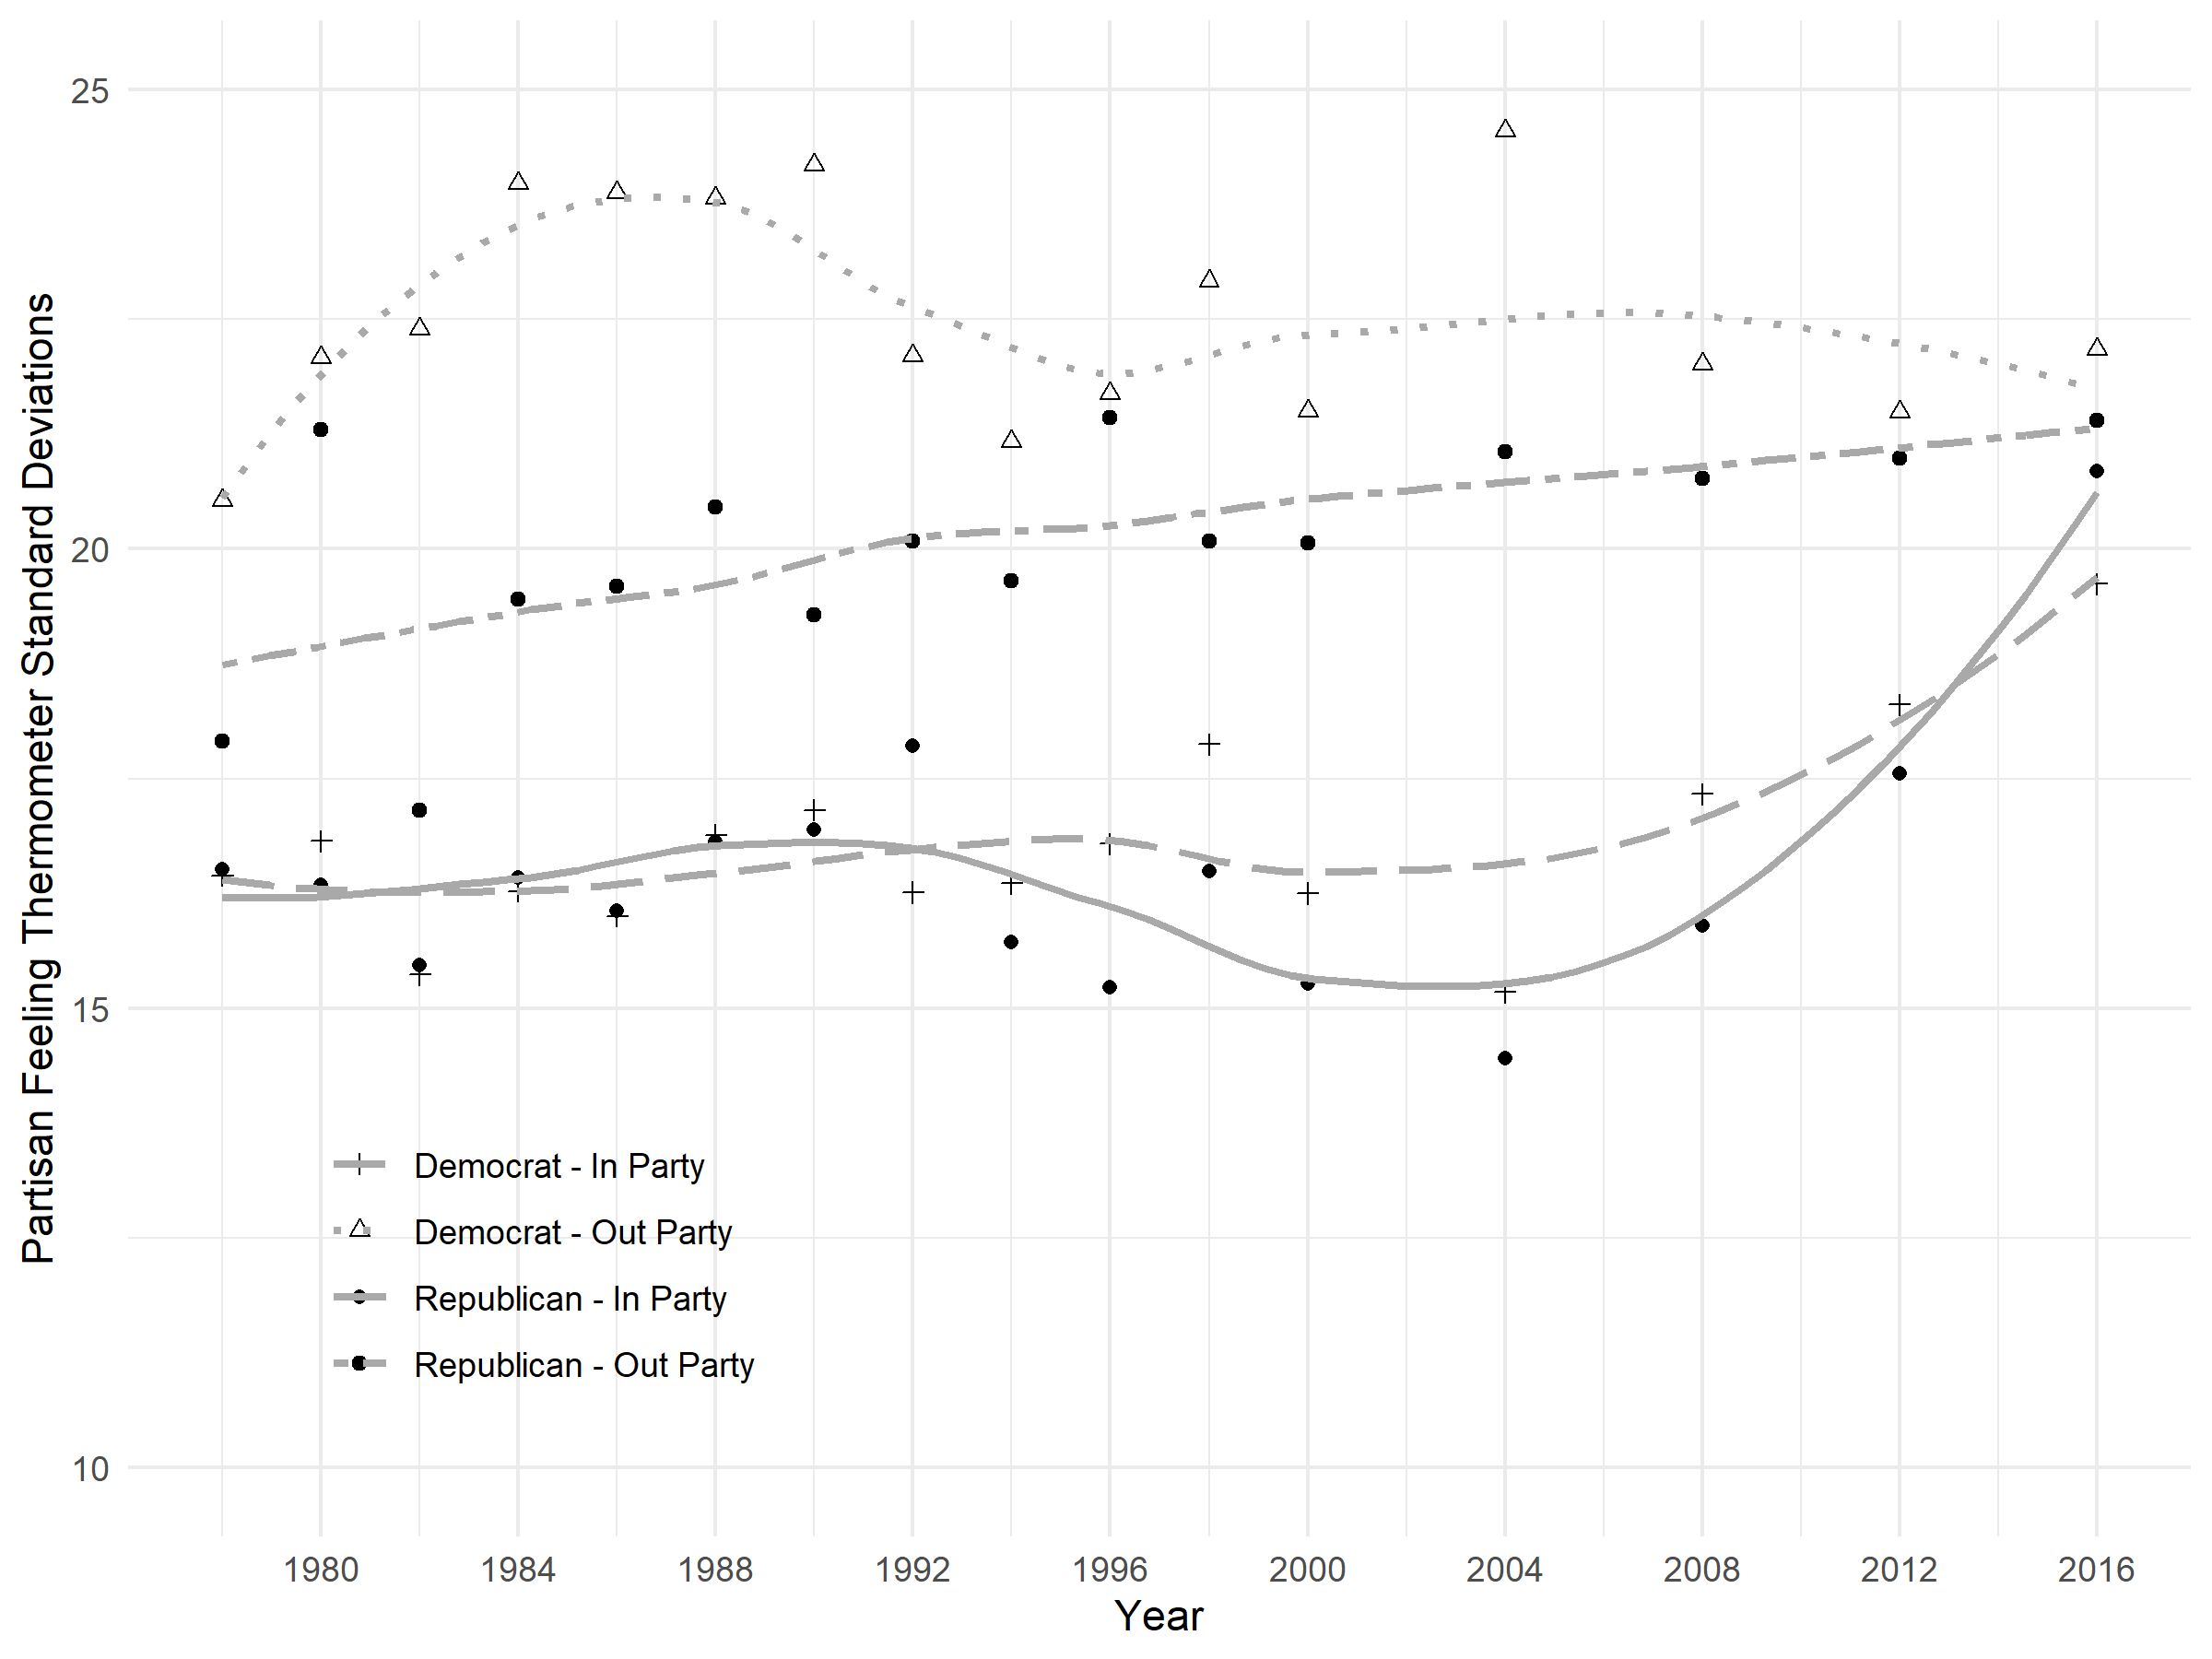
\includegraphics[width=5in]{cdf-sd.png}
\caption{\label{fig:cdf-sd} \textit{\textbf{Standard Deviation of partisans' in party feeling thermometers as reported in the ANES, 1978--2016.} After several decades of minimal change, the variation in in-party feeling thermometer ratings increased substantially between 2004 and 2016. This change is robust to both the Fligner-Killeen and Levene's tests of homogeneity of variance.}}
\end{figure}

Since 2004, partisans' feelings towards their own party have become less cohesive. This trend is less meaningful in regards to out-party feeling thermometers. While  the variance of out-party scores is similar in size to that of the in-party, out-party feeling thermometers have historically had high variance, particularly among Democrats.

Factions in both parties have received a great deal of attention in recent years. Groups like the Tea Party and alt-right in the Republican Party and progressives and socialists in the Democratic party have presented substantial challenges to their party's status-quo, often acting in opposition to their party's elites. Recent scholarship too has shown that affective divisions in the parties are both salient and predictive of other traits in partisans \citep{wronski2018tale, bankert2020authoritarian}. When the dependent variable in studies of polarization includes by default feelings towards the in-party, it becomes impossible to study how the effects of in-party feelings themselves have changed over time, or even to determine if they have any effect at all.


I hypothesize that, as partisans have become less consistent in their feelings towards their party there in-party feeling thermometers will be inconsistently related to their feelings towards the out-party. This hypothesis suggests that contemporary conceptions of political polarization, which presuppose that those who feel most warmly toward their co-partisans will  on average feel most coldly toward the opposition are subtly incorrect---it is not necessarily that partisans are warm towards their party and cold to the other. They are perfectly capable of being cold towards both groups. 

Further, I hypothesize that by controlling for in-party warmth, the modeled effect of cultural and economic attitudes will be more significant. When NPA is used as the dependent variable, the attitudes respondents who feel outside the ideological bounds of their party may cause them to report colder thermometers for both their in-party and out-party, which would not be detected by the NPA measure.

\subsection{Data \& Methodology}

By and large, the variables included in this extension are identical to those of the replication, with three major exceptions. Rather than a dependent variable calculated as the difference between in and out-party thermometers, I regress the model solely on out-party feeling, therefore, negative coefficients indicate that an increase in the variable causes the average respondent to dislike members of the out-party. In addition to the change of dependent variable, I include the in-party feeling thermometer as a covariate. Finally, I remove the dummy variable ``Strong Partisan" from the analysis to avoid overcontrol bias. The inclusion of that variable would block a path from warmth toward the in-party, causing the model to underestimate the effect of warmth towards the in-party on warmth towards the out-party. The equation for the models in this extension is:
\begin{equation}
\begin{split}
\hat{\mathit{Outparty Warmth}} = \alpha + \hat{\beta}_1{\mathit{Culture}} + \hat{\beta}_2\mathit{Econ} + \hat{\beta}_3\mathit{Inparty Warmth} +  \hat{\beta}_4\mathit{Interest} +  \gamma_5\mathit{Female} + \\ \hat{\gamma}_6\mathit{South} + \hat{\gamma}_7\mathit{High School} + \hat{\gamma}_8\mathit{Some College} + \hat{\gamma}_9\mathit{Adv. Deg.}
\end{split}
\end{equation}
each variable is coded to be between [0, 1] following the same guidelines as the replication.
\subsection{Results}
My first hypothesis, that the effect of warmth towards one's in-party should be less in 2016 than in 1988 or 2004 is largely supported by these results. While Democrats do see a significant effect of in-party affect in 2016, the magnitude of this effect is fairly small compared to previews years, and Republicans experienced no effect at all.

Additionally, cultural and economic attitudes are more frequently shown to have an effect on out-party thermometers when controlling for in-party feelings than in the replication model. This offers some support to my second hypothesis, but it should be noted that the magnitude of these effects are fairly small (and in the case of Democrats in 2016, decreased between the replication and extension models). Nonetheless, these results indicate that the forces
% Table created by stargazer v.5.2.2 by Marek Hlavac, Harvard University. E-mail: hlavac at fas.harvard.edu
% Date and time: Tue, Apr 21, 2020 - 3:25:31 AM
% Requires LaTeX packages: dcolumn 
\begin{table}[H] \centering 
  \caption{Original Models Using Outparty Affect as DV} 
  \label{} 
\begin{tabular}{@{\extracolsep{-10pt}}lD{.}{.}{-2} D{.}{.}{-2} D{.}{.}{-2} D{.}{.}{-2} D{.}{.}{-2} D{.}{.}{-2} } 
\\[-1.8ex]\hline 
\hline \\[-1.8ex] 
 & \multicolumn{6}{c}{Covariates of Out Party Affect} \\ 
\cline{2-7} 
\\[-1.8ex] & \multicolumn{2}{c}{1988} & \multicolumn{2}{c}{2004} & \multicolumn{2}{c}{2016} \\ 
 & \multicolumn{1}{c}{Dems} & \multicolumn{1}{c}{Reps} & \multicolumn{1}{c}{Dems} & \multicolumn{1}{c}{Reps} & \multicolumn{1}{c}{Dems} & \multicolumn{1}{c}{Reps} \\ 
\\[-1.8ex] & \multicolumn{1}{c}{(1)} & \multicolumn{1}{c}{(2)} & \multicolumn{1}{c}{(3)} & \multicolumn{1}{c}{(4)} & \multicolumn{1}{c}{(5)} & \multicolumn{1}{c}{(6)}\\ 
\hline \\[-1.8ex] 
 Cultural Attitudes & 0.01 & -0.07^{**} & -0.11^{**} & -0.05 & -0.09^{**} & -0.11^{***} \\ 
  & (0.03) & (0.03) & (0.05) & (0.04) & (0.04) & (0.03) \\ 
  & & & & & & \\ 
 Economic Attitudes & -0.19^{***} & -0.19^{***} & -0.21^{***} & -0.27^{***} & -0.30^{***} & -0.29^{***} \\ 
  & (0.04) & (0.04) & (0.05) & (0.05) & (0.06) & (0.05) \\ 
  & & & & & & \\ 
 In-Party Warmth & -0.19^{***} & -0.10^{**} & -0.18^{***} & -0.24^{***} & -0.10^{**} & -0.06 \\ 
  & (0.05) & (0.04) & (0.06) & (0.05) & (0.05) & (0.04) \\ 
  & & & & & & \\ 
 Political Knowledge & -0.001 & -0.03 & -0.16^{***} & -0.04 & -0.12^{***} & -0.20^{***} \\ 
  & (0.03) & (0.03) & (0.04) & (0.04) & (0.04) & (0.04) \\ 
  & & & & & & \\ 
 Gender: Female & 0.01 & -0.01 & -0.03 & -0.02 & 0.001 & -0.02 \\ 
  & (0.02) & (0.02) & (0.02) & (0.02) & (0.02) & (0.02) \\ 
  & & & & & & \\ 
 Region: South & 0.04^{**} & -0.04^{**} & -0.002 & 0.02 & 0.05^{**} & -0.01 \\ 
  & (0.02) & (0.02) & (0.02) & (0.02) & (0.02) & (0.02) \\ 
  & & & & & & \\ 
 Race: White & -0.01 & -0.03 & -0.05^{**} & -0.02 & 0.01 & -0.06^{**} \\ 
  & (0.02) & (0.03) & (0.02) & (0.03) & (0.02) & (0.02) \\ 
  & & & & & & \\ 
 High School & 0.002 & -0.04 & 0.13^{**} & -0.14^{**} & -0.02 & 0.01 \\ 
  & (0.03) & (0.03) & (0.06) & (0.07) & (0.06) & (0.14) \\ 
  & & & & & & \\ 
 Some College & -0.01 & -0.06^{*} & 0.10 & -0.12^{*} & -0.08 & 0.04 \\ 
  & (0.03) & (0.04) & (0.06) & (0.07) & (0.06) & (0.14) \\ 
  & & & & & & \\ 
 College/Adv. Degree & -0.03 & -0.07^{*} & 0.07 & -0.13^{*} & -0.11^{*} & 0.05 \\ 
  & (0.03) & (0.04) & (0.06) & (0.07) & (0.06) & (0.14) \\ 
  & & & & & & \\ 
 Constant & 0.73^{***} & 0.78^{***} & 0.80^{***} & 0.93^{***} & 0.82^{***} & 0.70^{***} \\ 
  & (0.06) & (0.05) & (0.09) & (0.08) & (0.08) & (0.14) \\ 
  & & & & & & \\ 
\hline \\[-1.8ex] 
Observations & \multicolumn{1}{c}{891} & \multicolumn{1}{c}{778} & \multicolumn{1}{c}{556} & \multicolumn{1}{c}{473} & \multicolumn{1}{c}{497} & \multicolumn{1}{c}{494} \\ 
Adjusted R$^{2}$ & \multicolumn{1}{c}{0.05} & \multicolumn{1}{c}{0.07} & \multicolumn{1}{c}{0.12} & \multicolumn{1}{c}{0.14} & \multicolumn{1}{c}{0.17} & \multicolumn{1}{c}{0.19} \\ 
\hline 
\hline \\[-1.8ex] 
\textit{Note:}  & \multicolumn{6}{r}{$^{*}$p$<$0.1; $^{**}$p$<$0.05; $^{***}$p$<$0.01} \\ 
\end{tabular} 
\end{table} 

\noindent driving partisan hostility may not be as simple partisan identity and economic opinions, clearly important though these variables are.
\section{Conclusion}
The main lesson of this study to scholars of political polarization should be the importance of clearly conceptualizing what is substantively important about polarization, and understanding the methodological trade-offs that occur when too much is built in to our dependent-variable models of polarization. The tacit (or explicit) assumption that in-party feelings are necessarily high when out-party feelings are low should be put to rest.

Given that partisans feelings towards their own party are not necessarily predictive of their feeling toward the opposing party, political scientists should carefully consider what substantive questions they are interested in asking when justifying a choice of dependent variable, recognizing that choice can limit the number of questions which can be asked, and obscure potential insights.

If scholars' interest in affective polarization is truly in the distance between partisans' assessments of themselves and their opponents, a measure like net partisan affective is appropriate. If, however, the researcher's interest is in the absolute political hostility or animus \textit{implied} by that distance, they should simply use partisan's direct feelings towards their enemies. There is no reason for those in the latter camp to run the risk of overcomplicating an analysis or confounding an interesting result by including in their measure a variable unrelated to their interests.
%\subsection{Research Design Concerns and Limitations}
%\begin{figure}[H]
%\center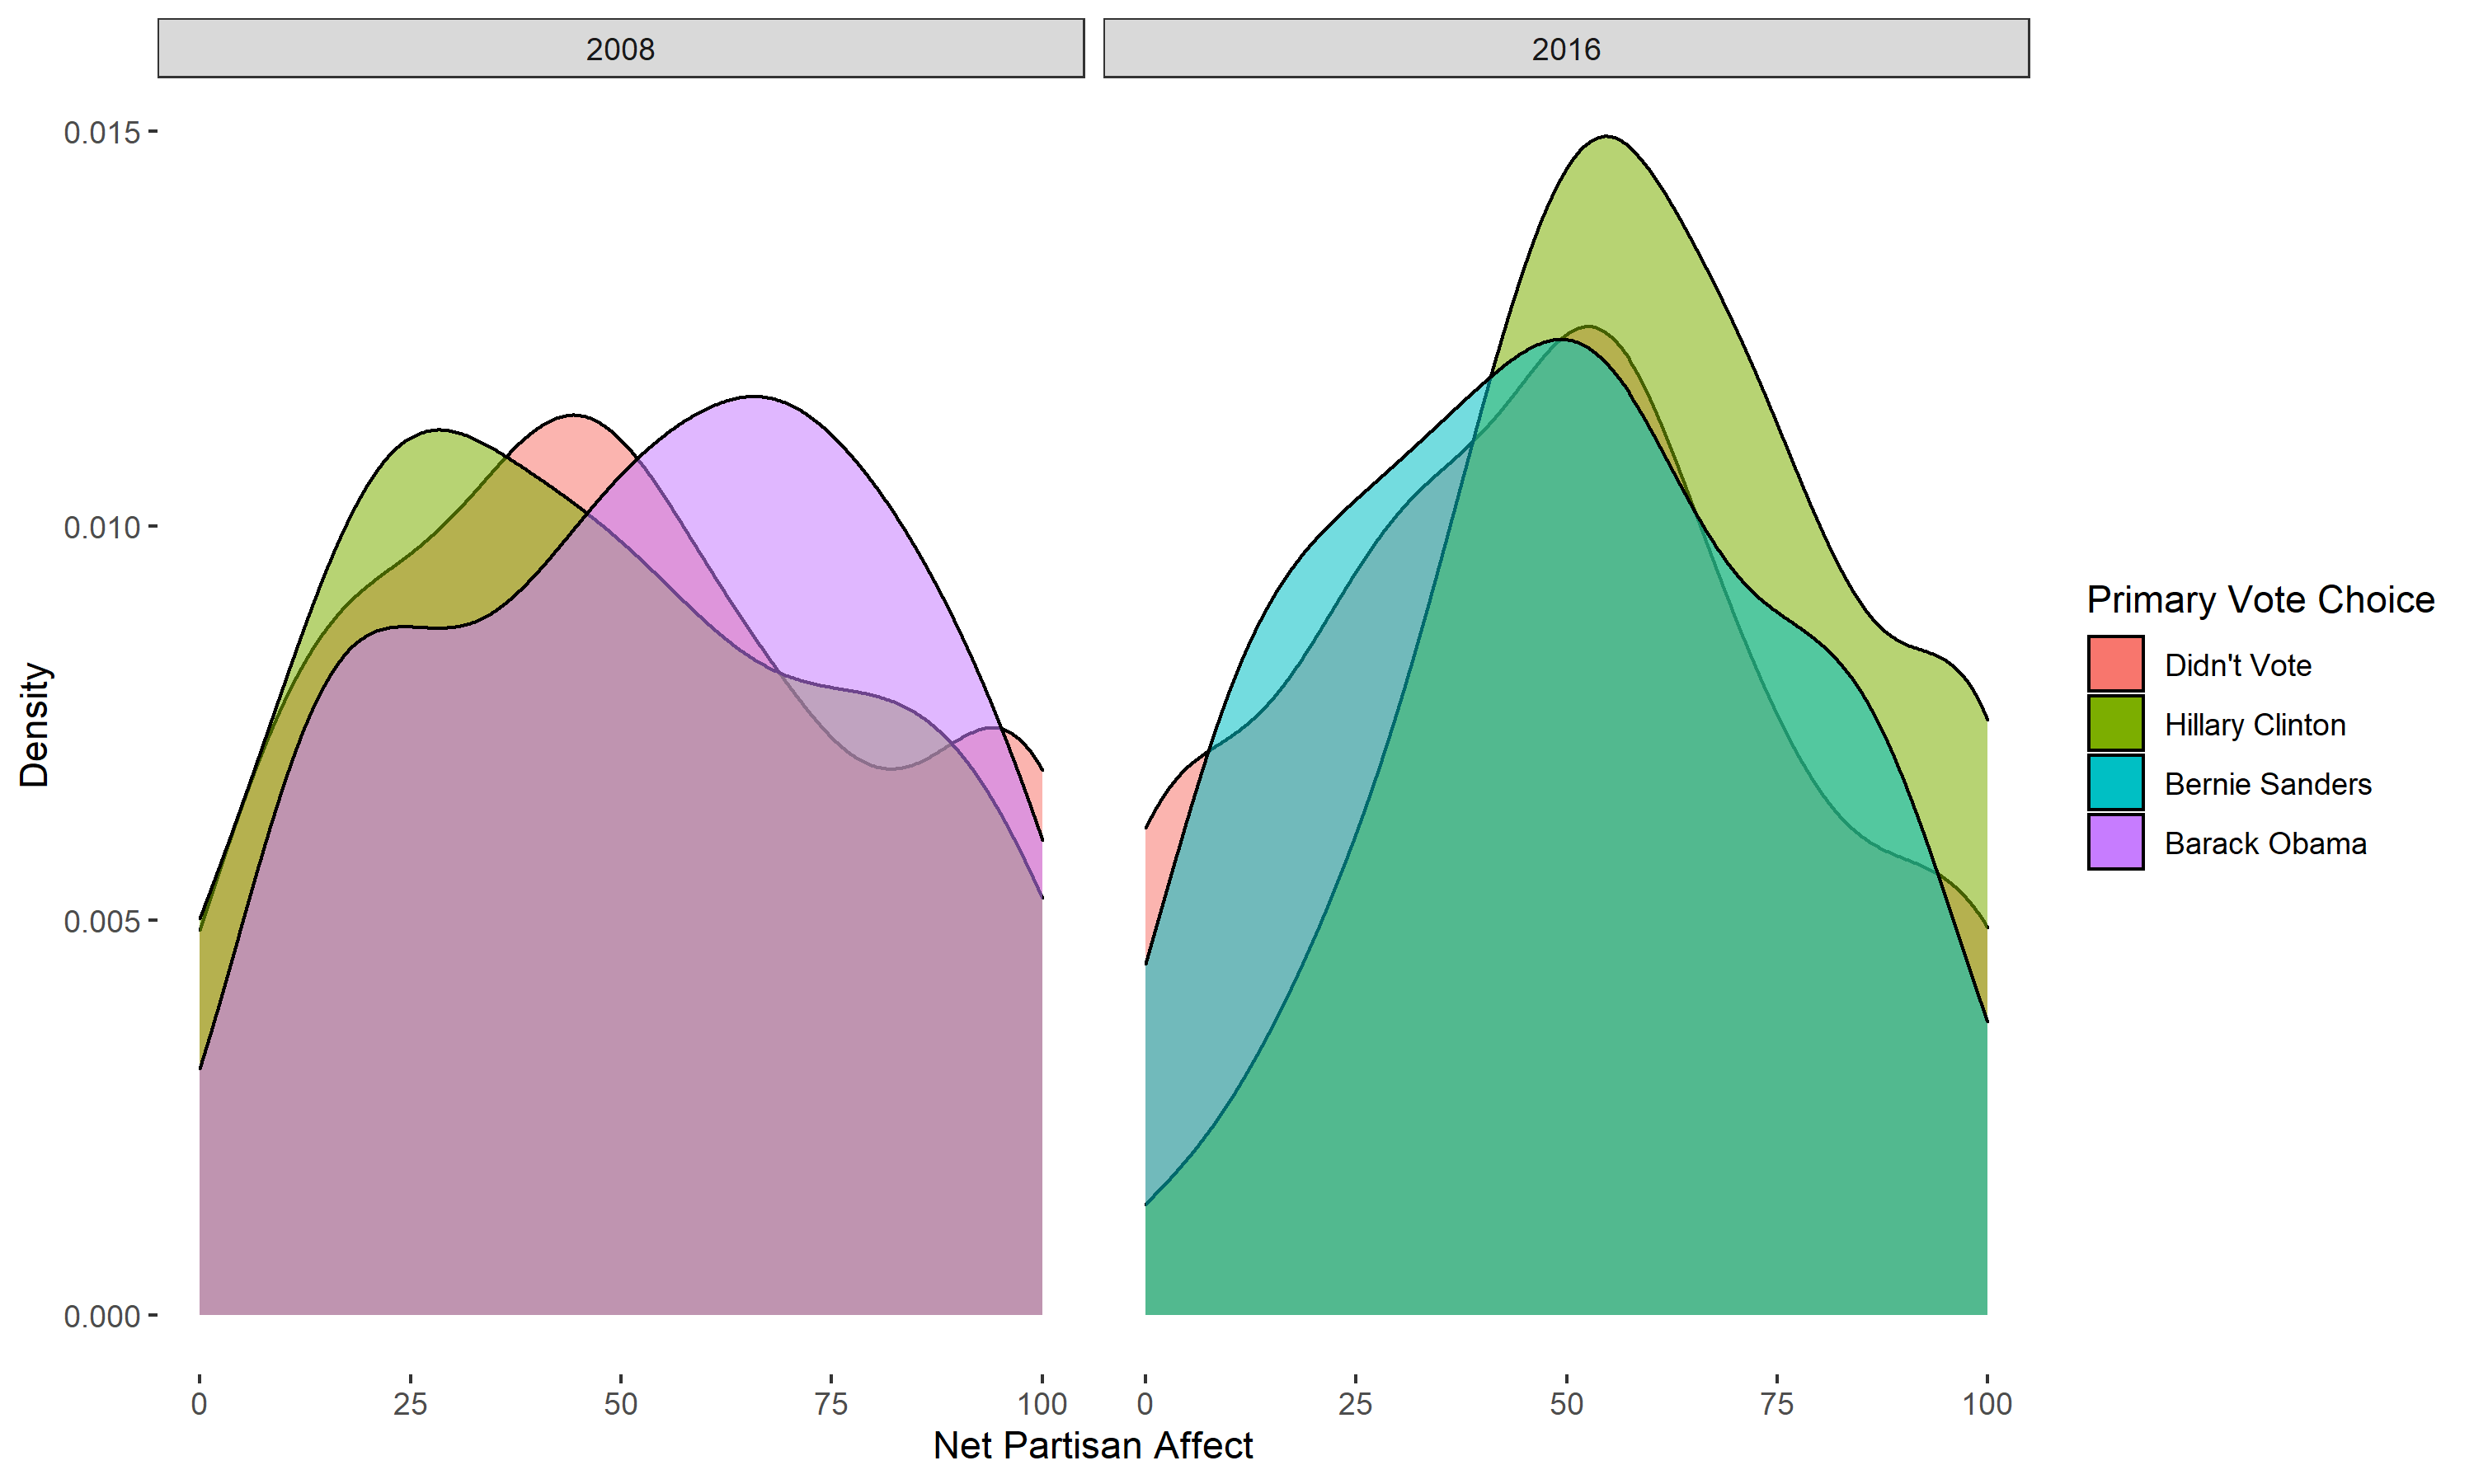
\includegraphics[width=6in]{therm-hist-2016.png}
%\caption{\label{fig:dens}\textit{Density plots of net partisan affect by vote in primary elections}.}
%\end{figure}

%These data are obviously quite limited, looking at members of one party across two years, but they should motivate additional research.


%compare decrease in NPA of losers to average NPA decrease of losers.



\thispagestyle{empty}
\clearpage
\setstretch{1}
\bibliography{references}
%\section{Appendix}



%\subsection{ISL's Model Extended to 2016}



%
%\section{Intra-Party Affect \& Primaries}
%
%In this section, I motivate an extension to \citet{iyengar2012affect}, drawing on partisanship and feeling thermometer data from the ANES-CDF to present time-series trends in Democrats' affect toward their party and the Republican Party. I show, consistent with extant literature, mean out-party feeling thermometers have been decreasing since the late \nth{20} Century. However, the mean feeling thermometers of the parties writ-large do not provide a sufficiently nuanced view of citizens' affect.
%
%\subsection{Internal Division}
%Extant scholarship has, in large part, treated the major parties as affectively monolithic; party ID is assumed the least common denominator of political identity. It is also commonly assumed that warmth toward the in-party is (and has been) high across all partisans \citep{iyengar2012affect}. 
%
%
% While affective polarization between partisans \textit{is} very high at present, there is also reason to be suspicious of internal divisions \textit{within} each party. \cite{mason2018ideologues} finds that, in addition to partisan identity, citizens hold ideological identities. In other words, individuals see themselves not just as ``Democrats" and ``Republicans", but as ``liberals" and ``conservatives". These  ideological and partisan identities are related to one another, but suggest that political identities which cross cut partisanship are theoretically plausible.
%
%%\begin{figure}[H]
%%\center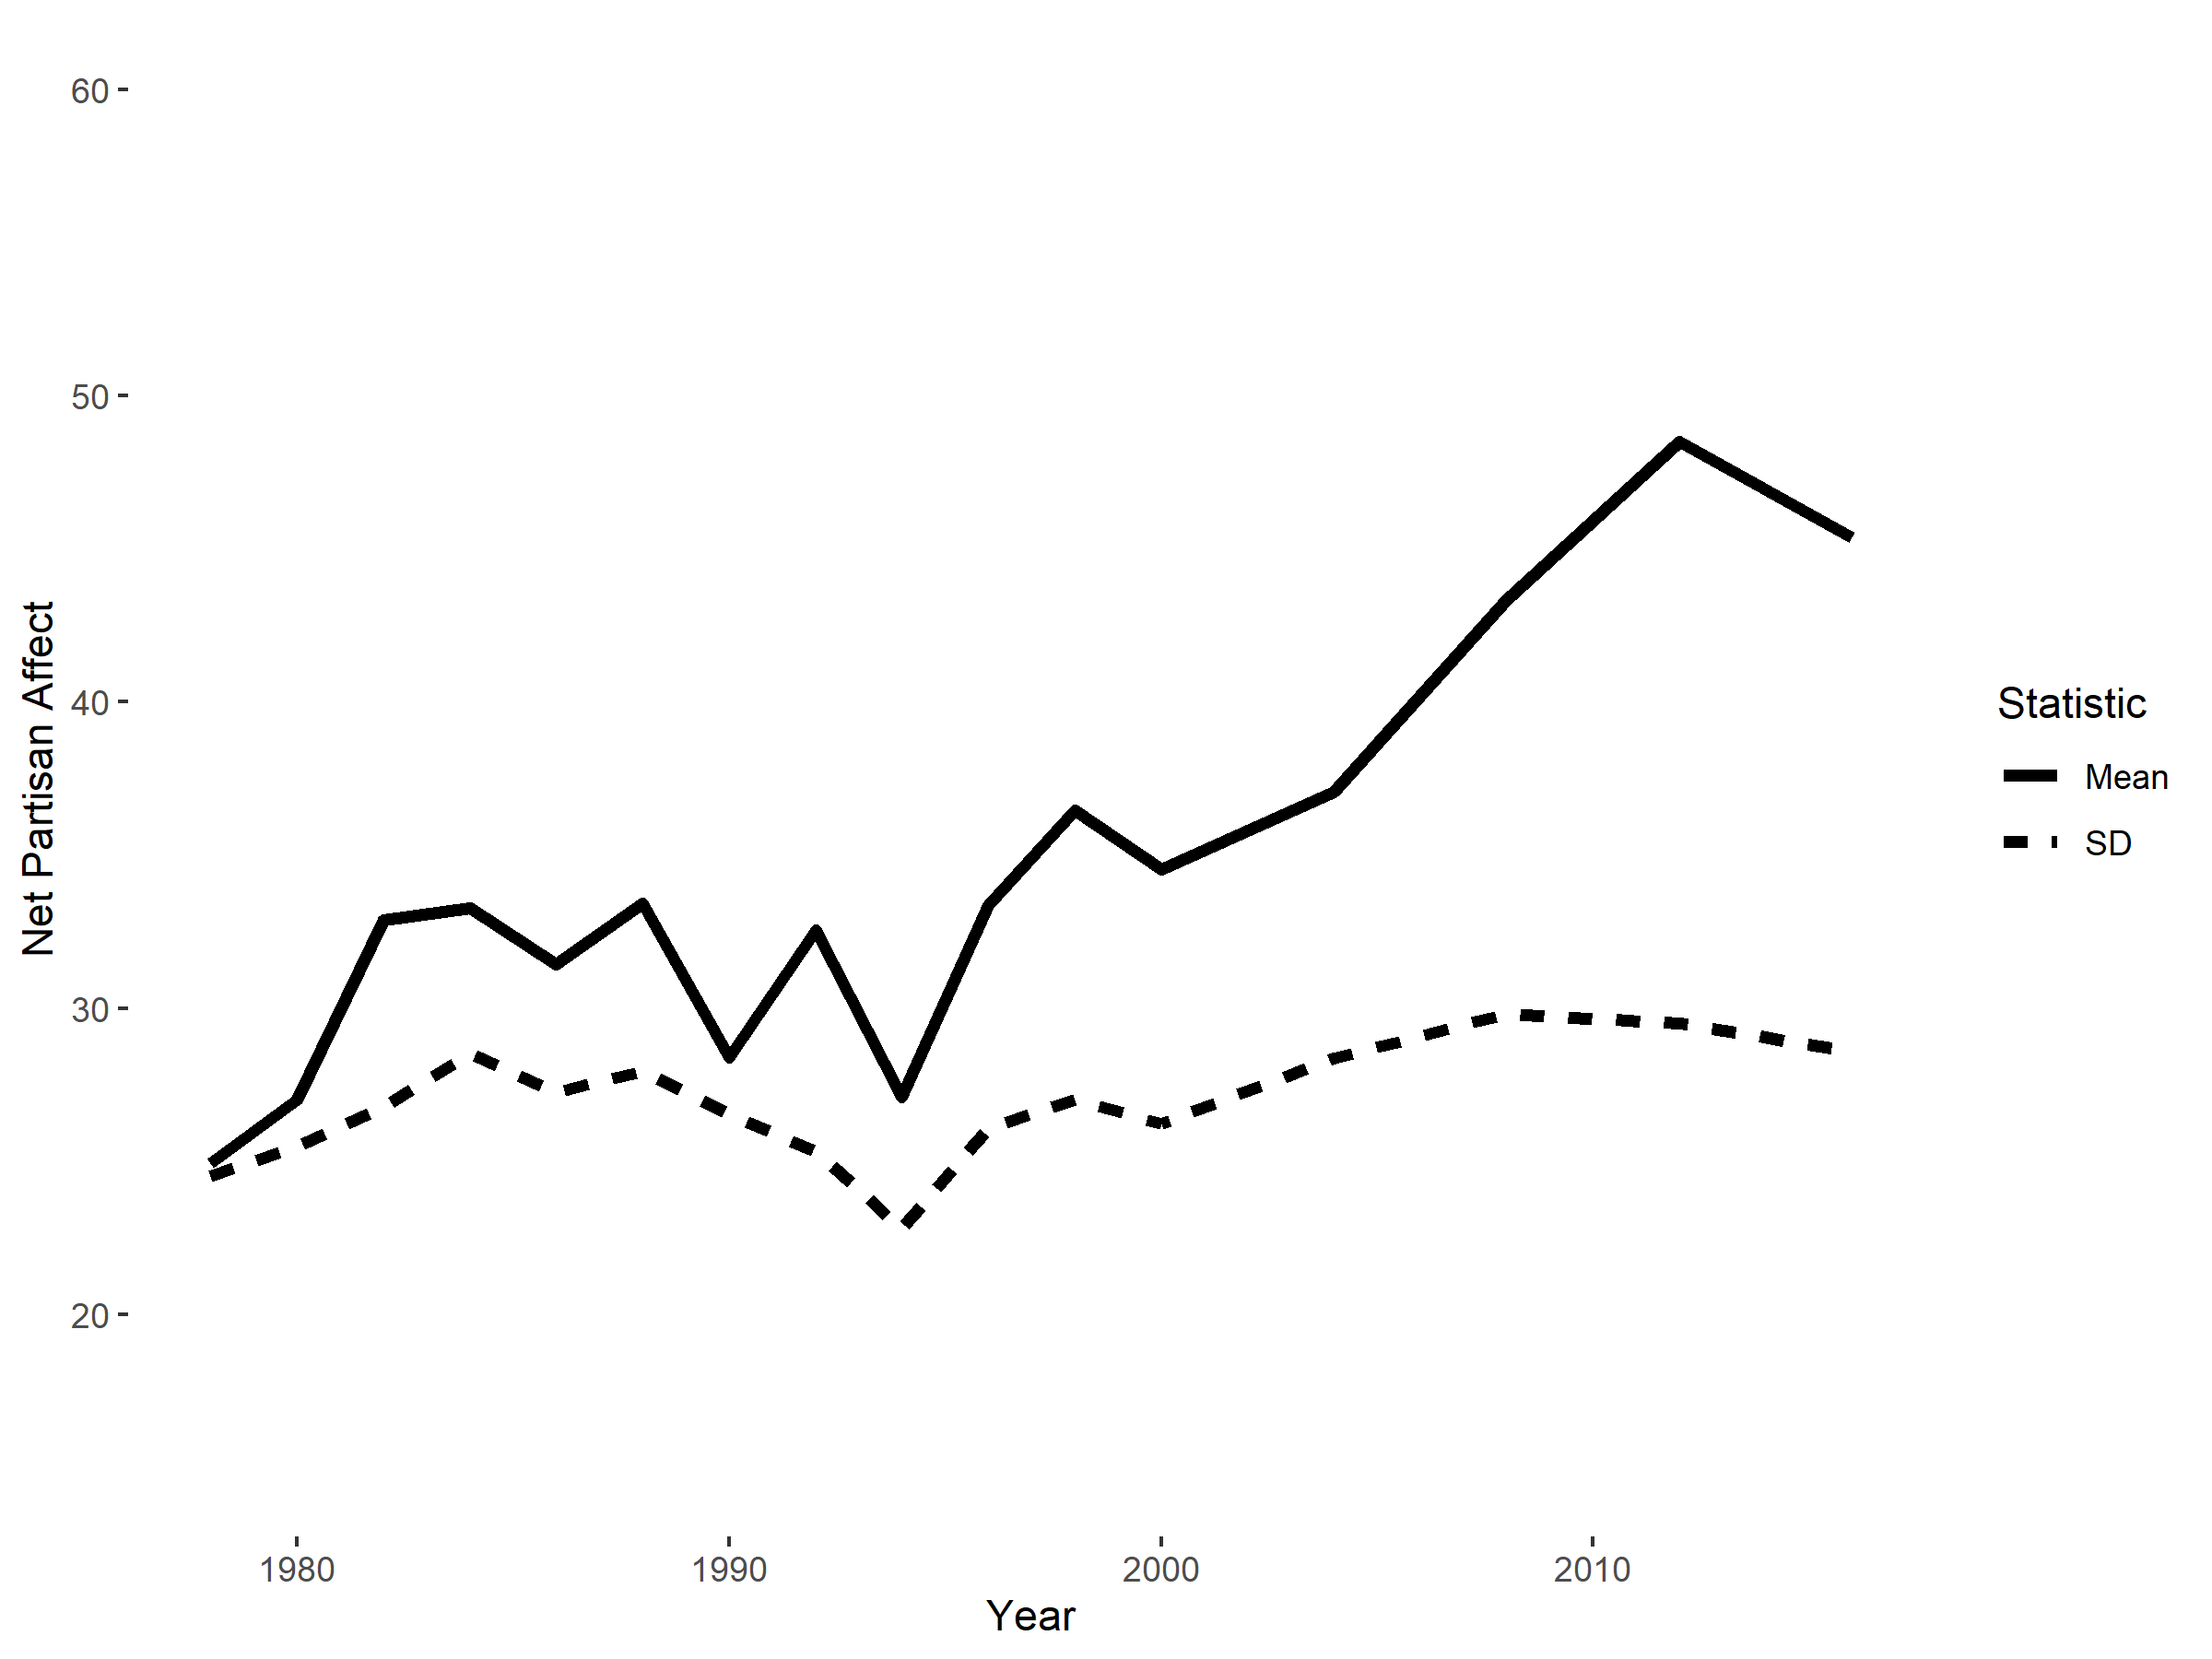
\includegraphics[width=6in]{cdf-npa.png}
%%\caption{\label{fig:cdf-npa} \textit{\textbf{Democrats Net Partisan Affect Since 1978.} NPA has increased, but so has the variance. Subtracting in-party FT from out-party FT obscures variation occurring in each measure.}}
%%\end{figure}
%\begin{figure}[H]
%\center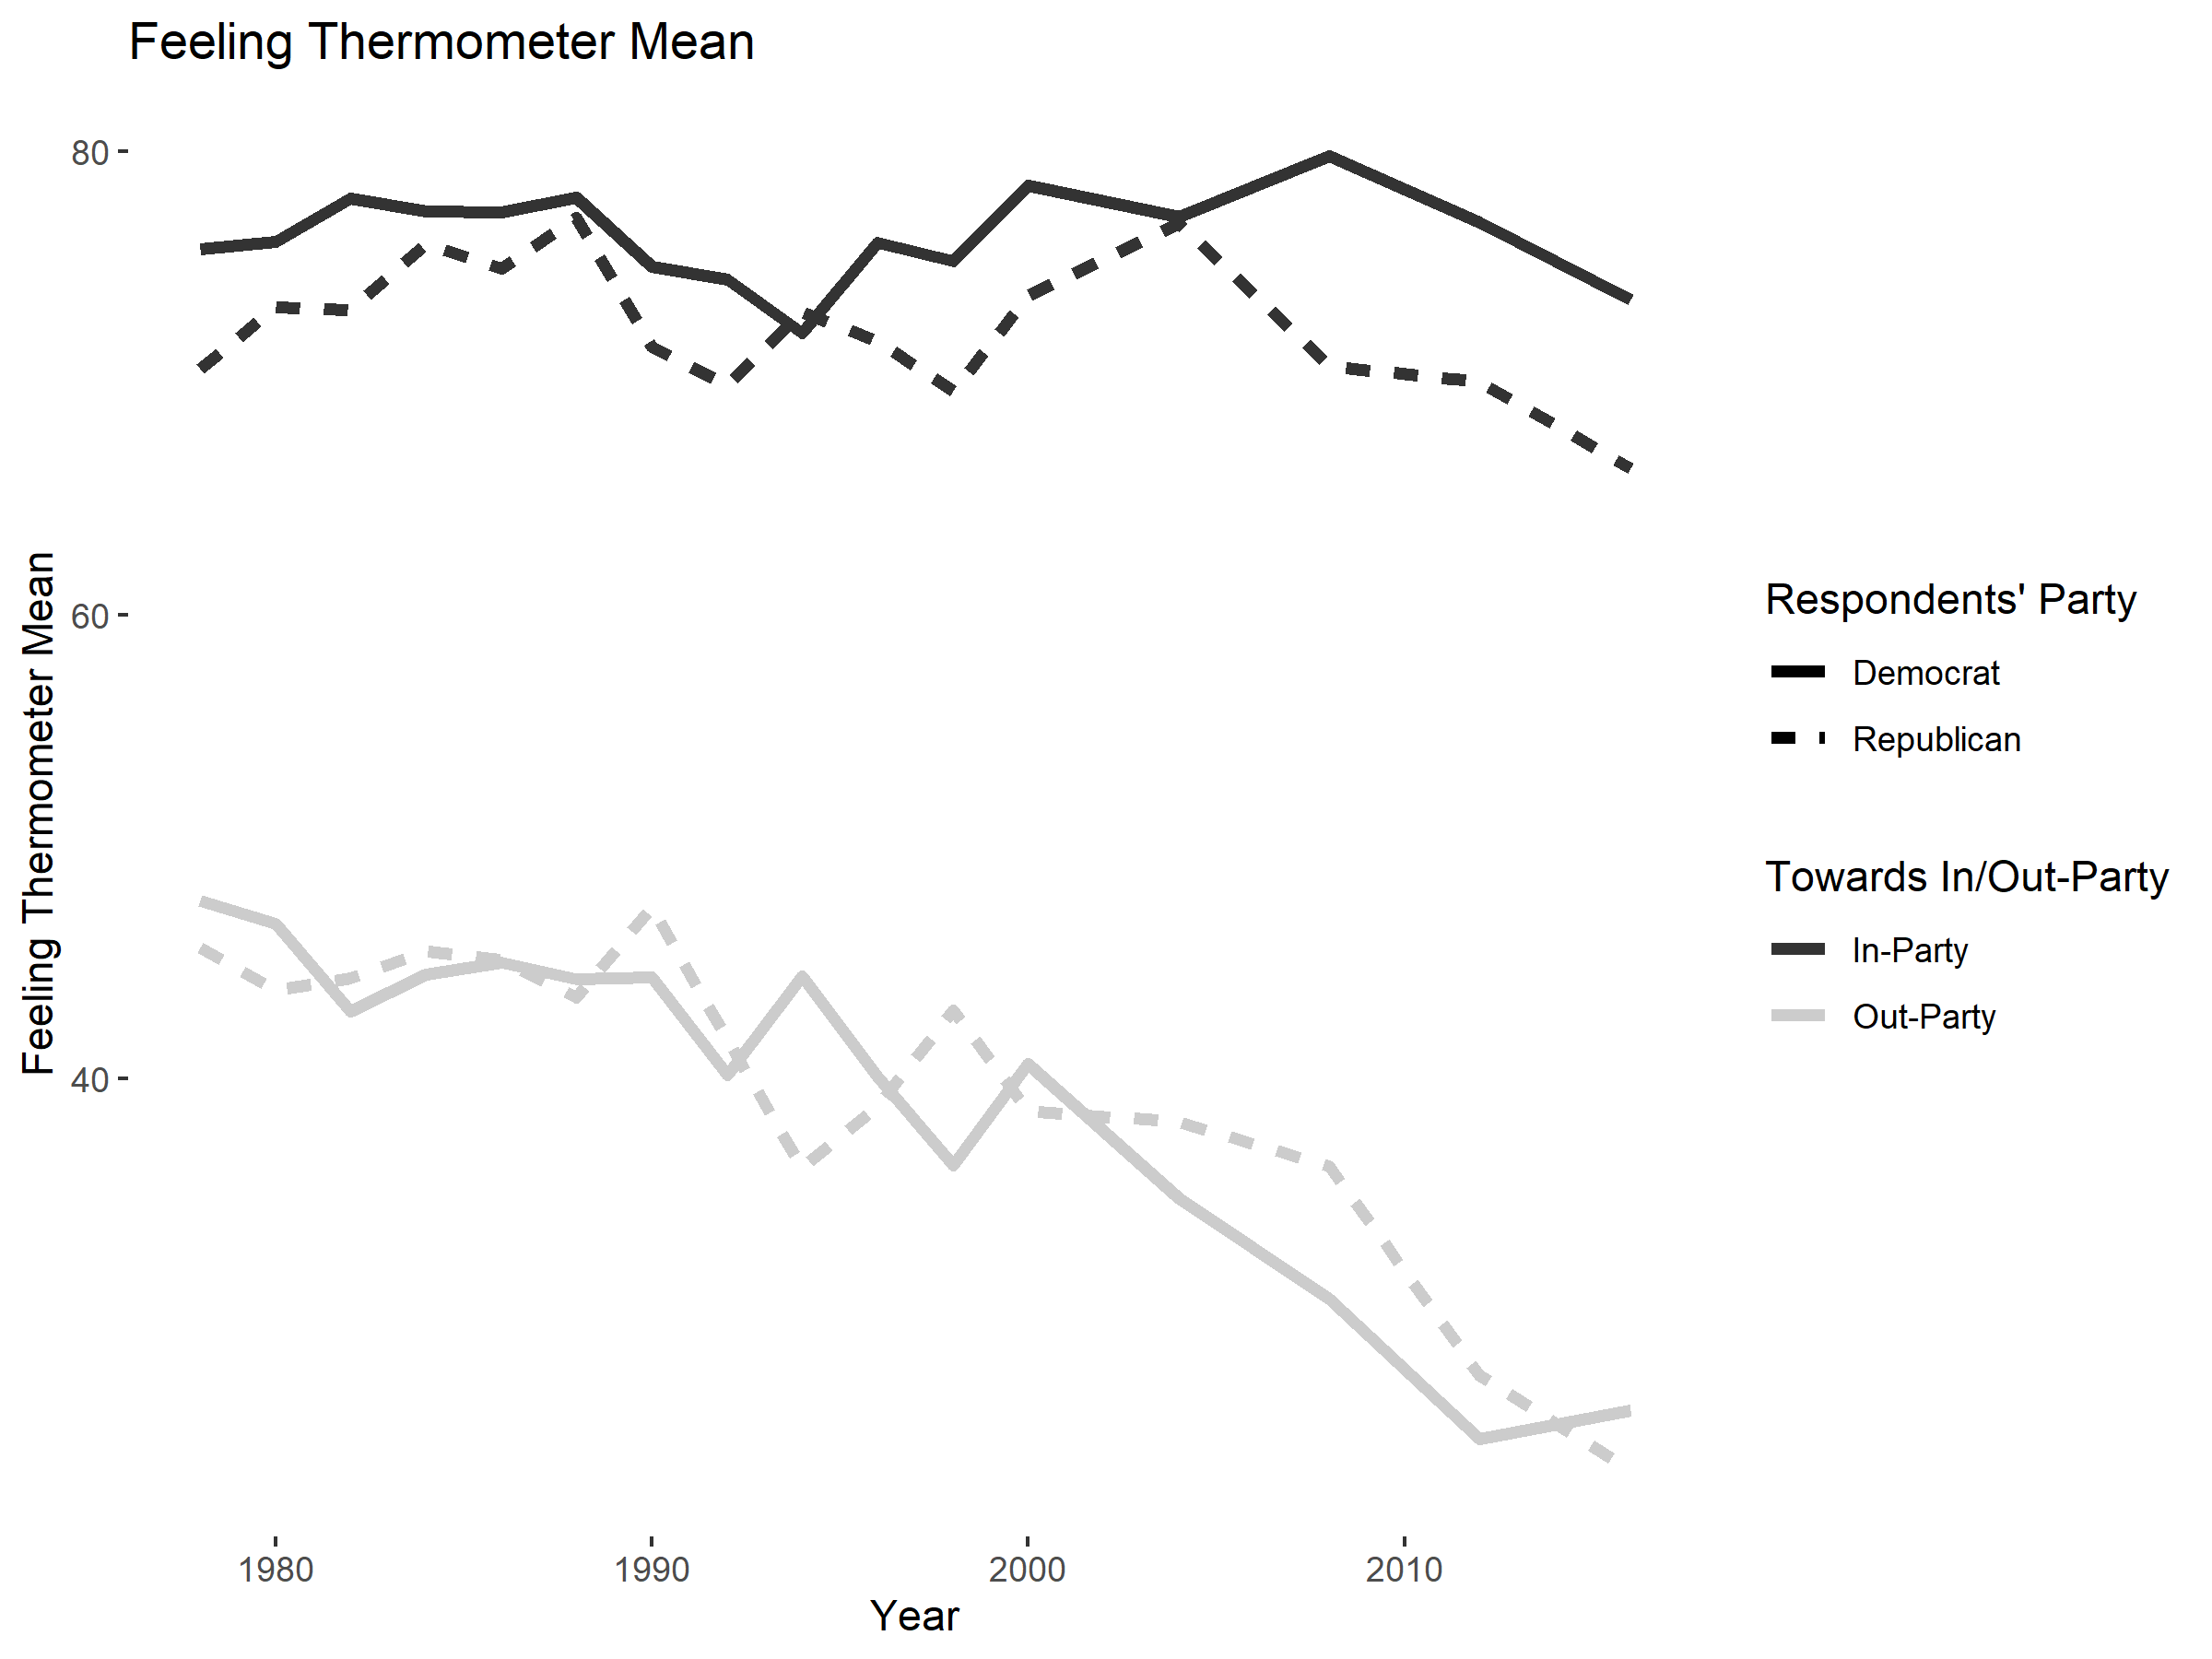
\includegraphics[width=5in]{cdf-avg.png}
%\caption{\label{fig:cdf-avg}\textit{\textbf{Yearly mean of partisans' in-party and out-party feeling thermometers, 1978--2016.} Consistent with the extant literature (e.g., \citet{iyengar2012affect}, Democrat and Republican in-party FTs are consistently high (with a slight decrease since the first decade of the 2000s).}}
%\end{figure}
%\noindent Figure \ref{fig:cdf-avg} shows the average in-party and out-party feeling thermometer for Republicans and Democrats from 1978-2016. We clearly see out-party feeling thermometers scores decline; while the in-party remains relatively constant. This is true of both parties.
%
%Unfortunately reliance on annual means as a description of partisan affect paints too simple a picture. The standard deviation of the feeling thermometers, presented in figure \ref{fig:cdf-sd}, shows that the stability of mean in-party affect observed in Figure \ref{fig:cdf-avg} belies an increase in the variation around that mean. This variation has increased in each iteration of the survey since 2004, both Republicans and Democrats have become less cohesive in their feelings toward their own party than at any other time period for which we have data. It should be noted that, historically, partisans are less cohesive in their feelings towards the out-party, though the variance in intra-party affect now seems to be on par with out-party feelings. %Both figures \ref{fig:cdf-sd} and \ref{fig:cdf-avg}are reproduced in the Appendix using data from Democrat leaning independents, to similar results.
%
%%%%%%%
%
%
%\begin{figure}[H]
%\center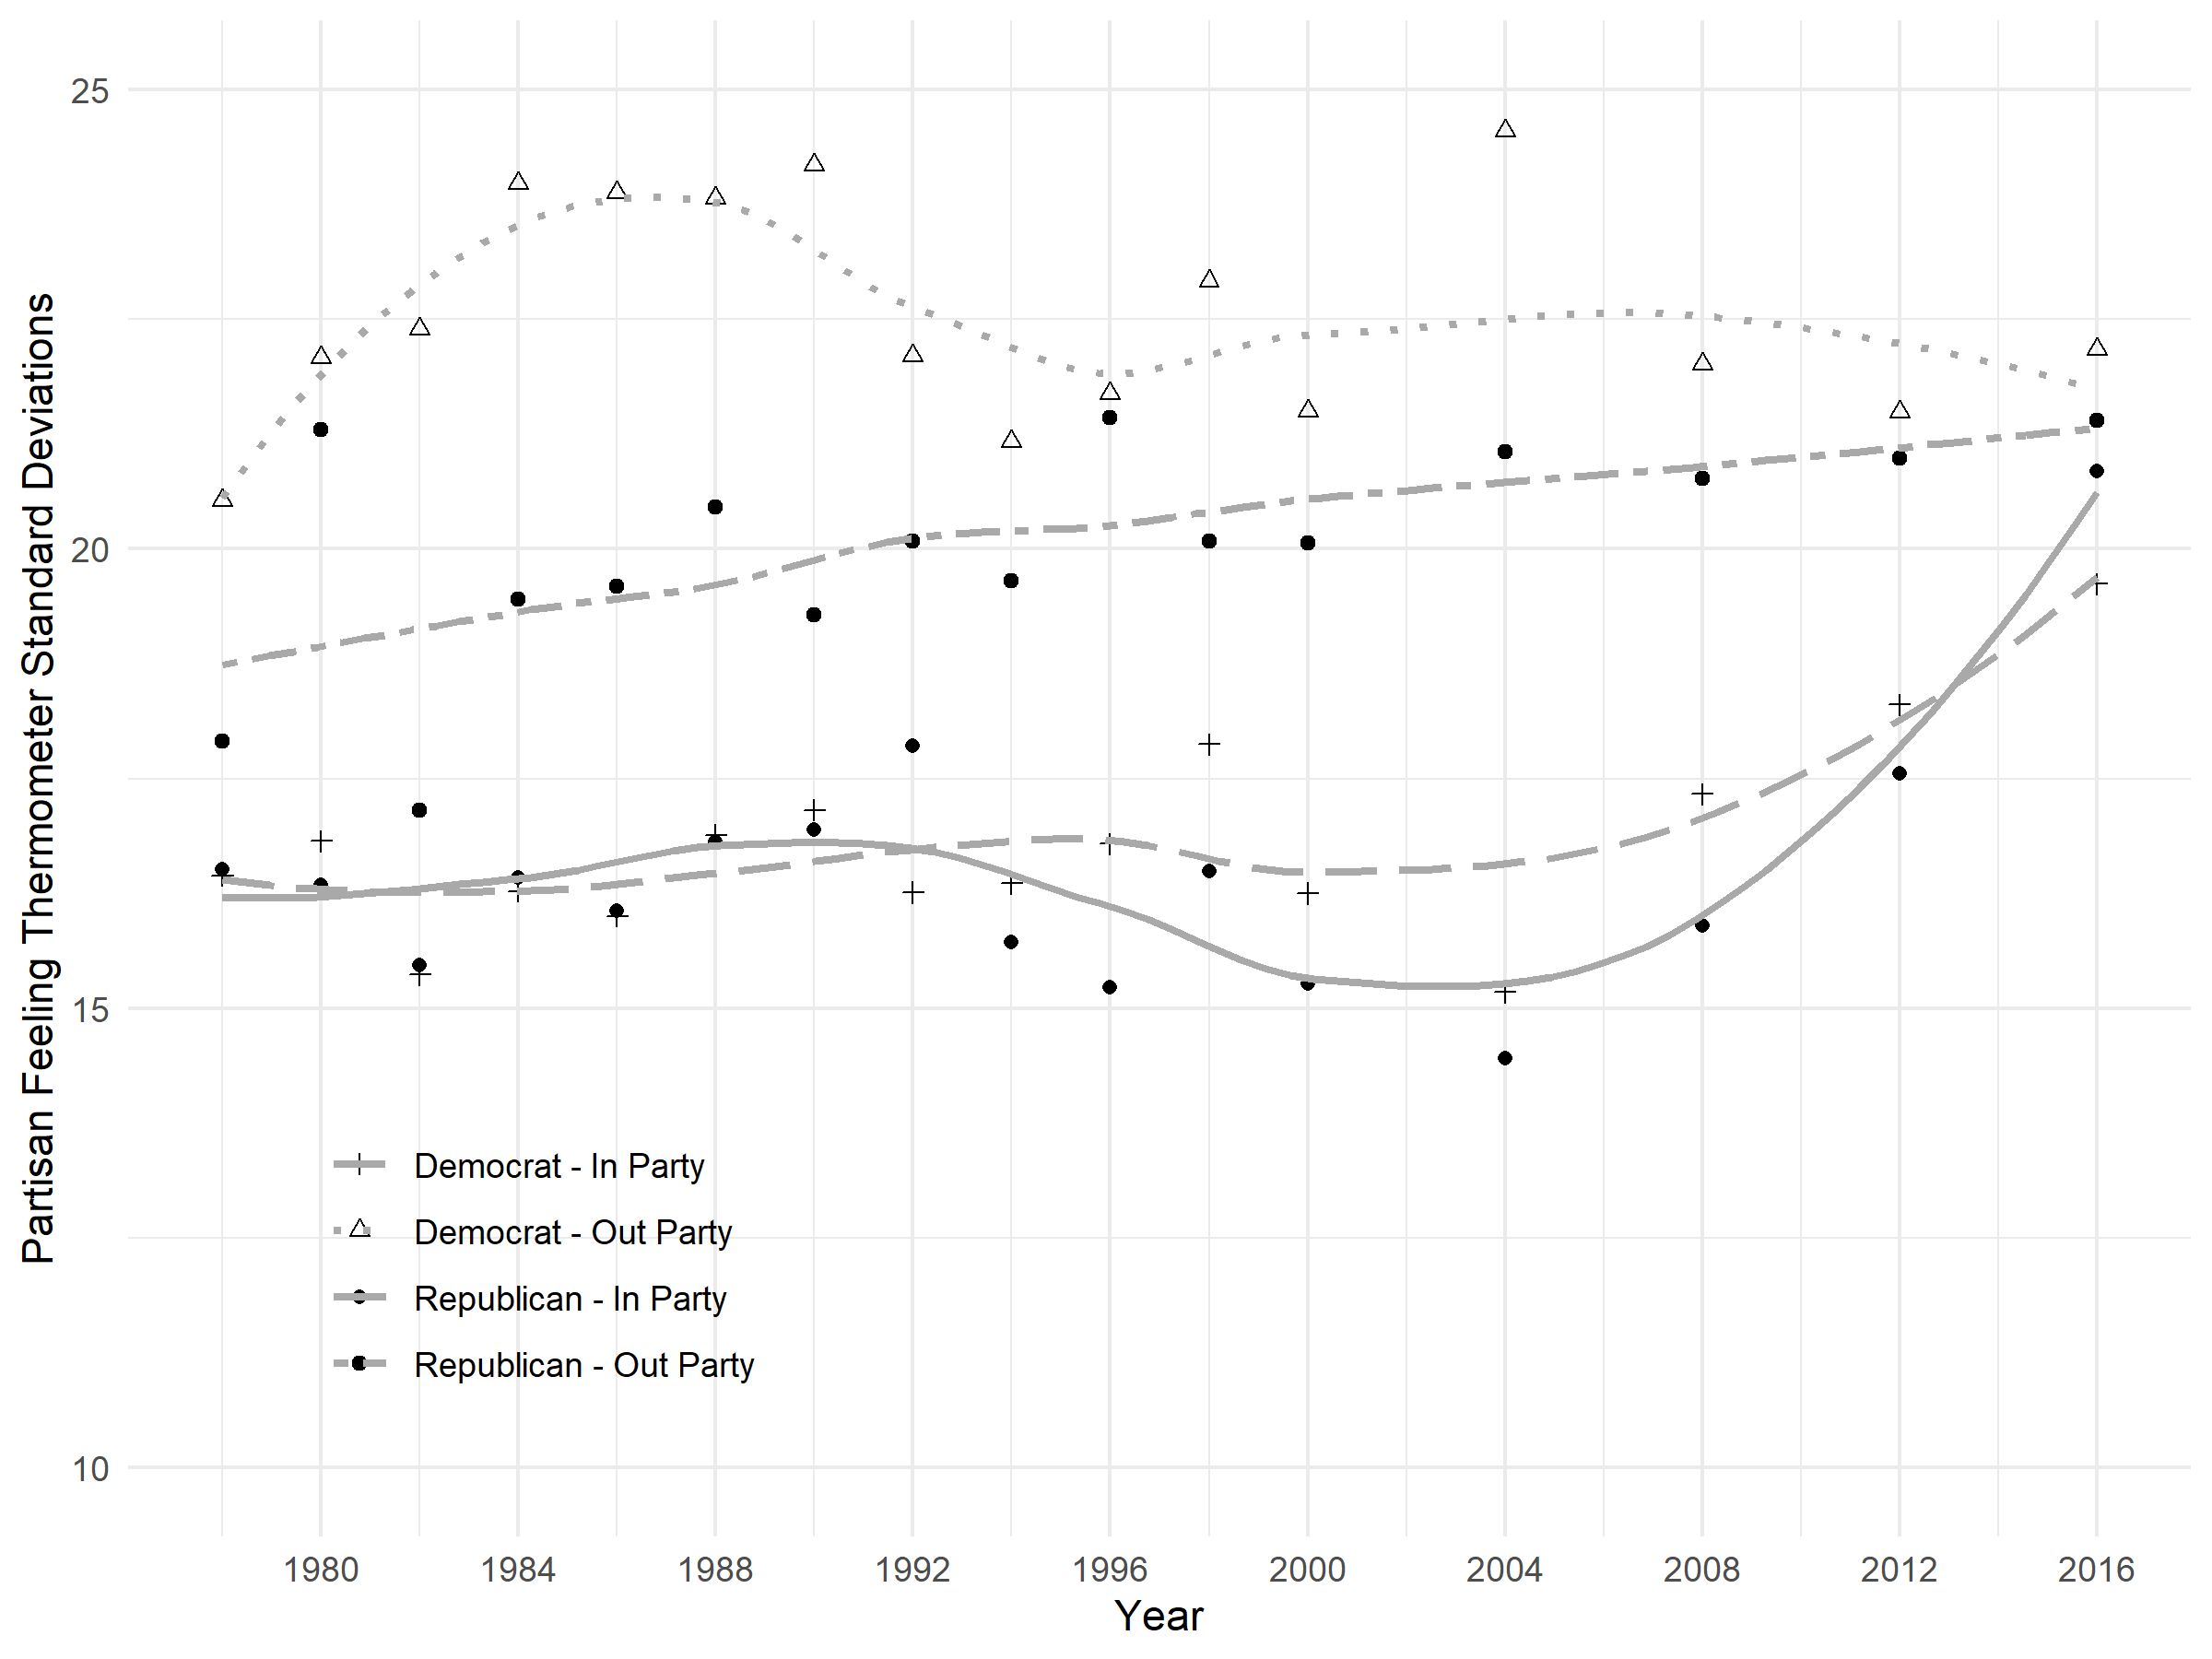
\includegraphics[width=5in]{cdf-sd.png}
%\caption{\label{fig:cdf-sd} \textit{\textbf{Standard Deviation of partisans' in party feeling thermometers, 1978--2016.} After several decades of minimal change, the variation in in-party feeling thermometer ratings increased substantially between 2004 and 2016. This change is robust to both the Fligner-Killeen and Levene's tests of homogeneity of variance.}}
%\end{figure}
%%%%%%
%
%
%
%The changes in variance observed above between 2004 and 2016, as well as 1978-2016 are robust to both the Levene's and Fligner-Killeen tests of homogeneity of variances. These tests evaluate the null hypothesis that the variance of a variable between two samples or groups is equal, and are robust to non-normally distributed data. Each tests rejects the null at $p<.05$ (precise p-values to be reported in the appendix).
%
%%\begin{figure}[H]
%%\center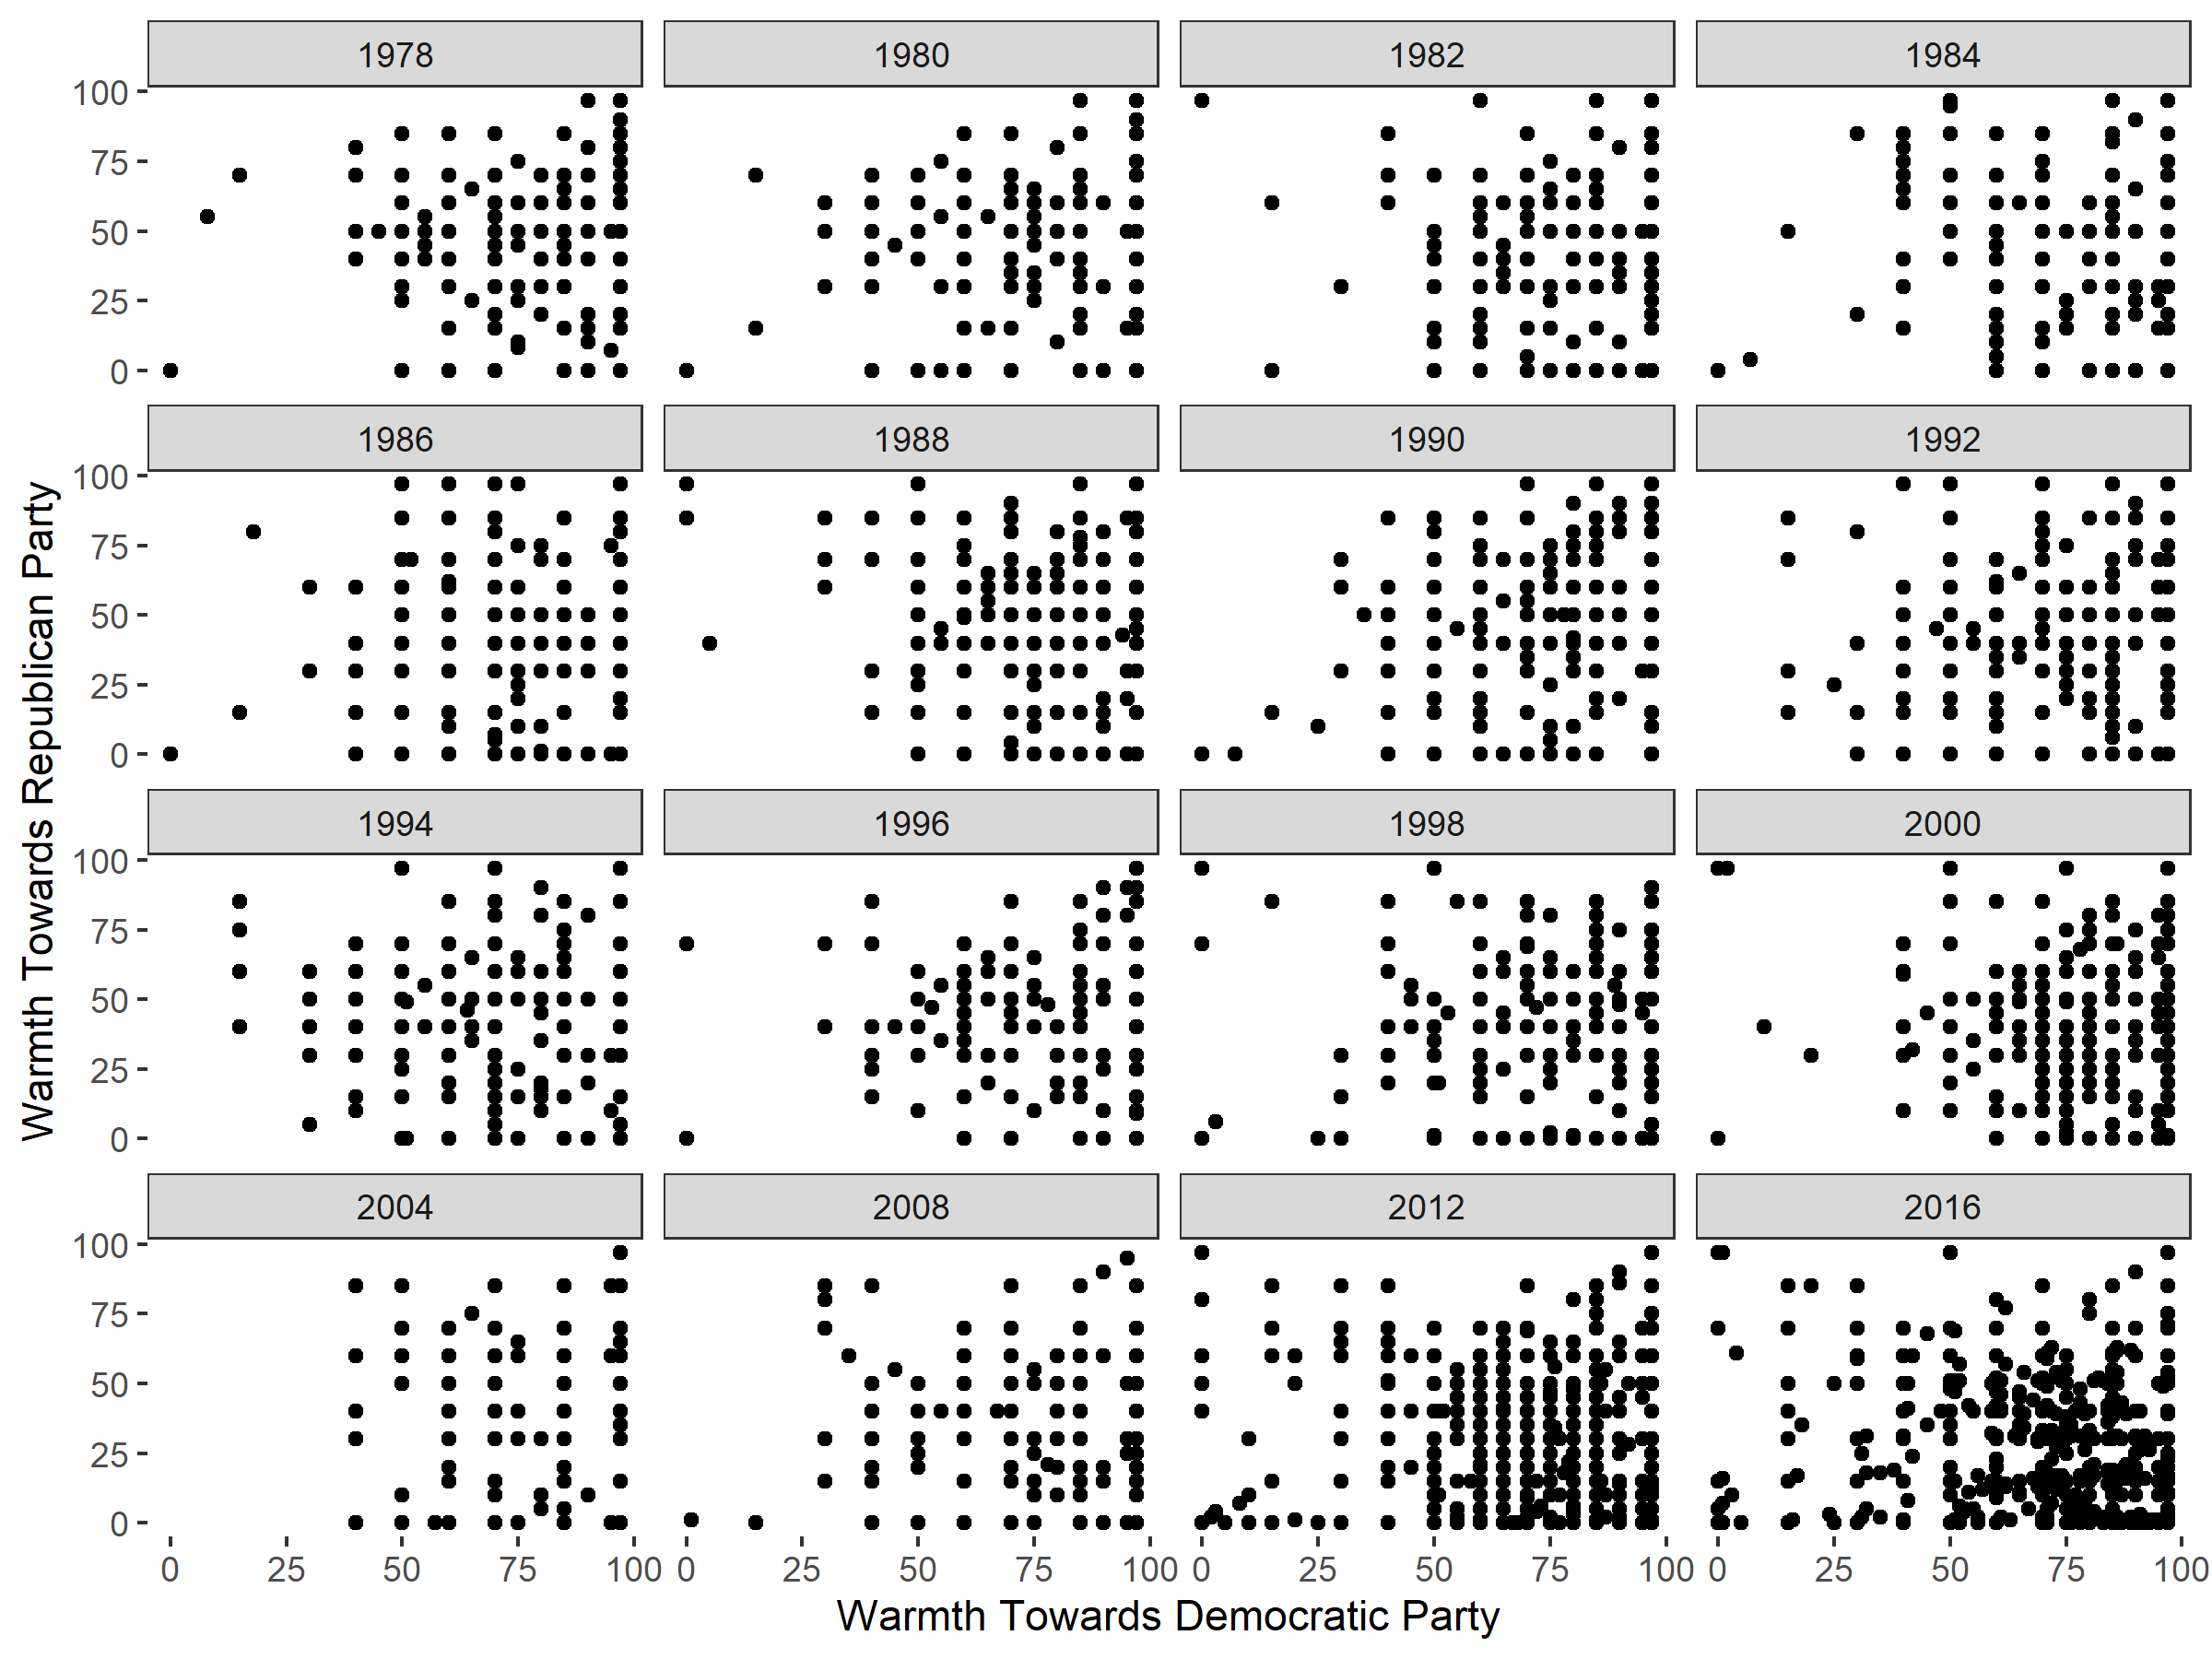
\includegraphics[width=6in]{cdf-scatter-dem.png}
%%\caption{\label{fig:cdf-scatter} \textit{\textbf{Scatterplots of Democrats' feeling thermometer scores toward the Democratic and Republican parties from 1978-2016.} Democrats have gotten more cold towards the Republican Party, but an increasing number are also cold towards \textit{both} parties.}}
%%\end{figure}
%
%%To visualize the variation described above, I scatterplot Democrats' feeling thermometers towards their in-party and out-party, across all available years. Consistent with the theoretical expectation of \cite{iyengar2012affect}, most respondents have clustered in the bottom right of the plot, indicating warmth towards the Democratic party and coldness towards the Republicans. However, in 2012 and 2016, we also see a striking number of respondents in the bottom left, reporting cold affect towards \textit{both} parties. 
%
%%Using a Levene Test---a statistical procedure which evaluates $H_0: \sigma_1 = \sigma_2$, I show that these data are sufficent to reject the null hypothesis stating that Democrat's in-party and out-party feeling thermometers displayed equal variation in 2004 and 2016. The increase in deviation from 2004, when Democrats were (in recent history) most cohesive, to 2016 at their most dispersed is unlikely to be due to chance. We reject the null hypothesis at $p < .001$, as indicated in the tabe below.
%
%%\begin{table}[H]
%%\begin{table}[H]
\centering
\begin{tabular}{>{\raggedright\arraybackslash}p{3cm}>{\raggedleft\arraybackslash}p{3cm}>{\raggedleft\arraybackslash}p{3cm}r}
\toprule
\textbf{ } & \textbf{Df} & \textbf{F value} & \textbf{Pr(>F)}\\
\midrule
group & 1 & 7.423141 & 0.0064838\\
 & 2501 & NA & NA\\
\bottomrule
\end{tabular}
\end{table}
%%\caption{\label{table-levene} \textit{\textbf{Results of a Levene Test on the 2004 and 2016 in-party feeling thermometers of Democrats, which indicates meaningful differences in the deviation of the feeling thermometers}}}
%%\end{table}
%\subsection{A Closer Look At Democrats}
%
%To assess the degree to which systematic differences in affect exist between members of party factions, I present sub-group analyses of primary voters. Primary elections are substantively significant events, allowing partisans a voice in the presentation and direction of their party. In a political environment in which the presidential nominee becomes the de facto leader of the party, the primary process affords non-elite voters a voice in the ideological, political, and stylistic future of the party. The political products offered by primary candidates may reflect (or drive) extant divisions in the party. \cite{wronski2018tale} and \cite{bankert2020authoritarian} find that those scoring highly on measures authoritarian personality traits use their primary vote to ``protect" their party from factions they see as threatening group cohesion. Just as voters do not toss a coin to decide their general election vote, they do not randomly select their choice in the primary; these choices are likely to be meaningful. 
%
%Journalistic accounts of primary elections and their aftermath abound with assertions of internal division and strife within parties after fraught primary election cycles. Democratic primary elections were surprisingly contentious in both 2008 and 2016. In 2008, a particularly brutal primary season spawned the ``Party Unity Means Action" movement (colloquially referred to as the ``Party Unity My Ass" movement) which culminated in an estimated 15-20\% of Clinton supporters voicing their support for John McCain in that year's general election\footnote{\url{https://www.washingtonpost.com/wp-dyn/content/article/2008/06/26/AR2008062604162_pf.html}}.
%
%In 2016 too, primary elections brought to light conflicts between the party's ascendant left-wing and party leadership. These primary divisions seemed to remain salient to engaged voters during the subsequent election for chair of the Democratic National Committee, where Keith Ellison, favored by Sanders supporters lost the race to Obama Secretary of Labor, Tom Perez. Staffers and executives of the 2016 Sanders campaign went on to create groups like \textit{Justice Democrats}, which supports left-leaning candidates in primaries against more centrist Democrats\footnote{Perhaps most notably: \textit{Justice Democrats} supported the campaign of Alexandria Ocasio-Cortez (D-NY), herself a former member of the 2016 Sanders campaign, against former representative Joe Crowley, a high-ranking establishment Democrat.}. 
%
%
%
%
% 
%
%\subsection{Differences in Affect Among Democratic Primary Voters}
%I turn now to subgroup analyses of participants and non-participants in the 2008 and 2016 Democratic primaries. I present data from the three largest categories of ANES respondents in each year. In 2008 these were supporters of Barack Obama and Hillary Clinton; in 2016, Hillary Clinton and Bernie Sanders. In each year non-voters made up a majority of respondents.
%\begin{table}[H]
%\begin{table}[H]
\centering
\begin{tabular}{ll>{\raggedleft\arraybackslash}p{3cm}>{\raggedleft\arraybackslash}p{3cm}>{\raggedleft\arraybackslash}p{3cm}>{}p{3cm}>{}p{3cm}>{}p{3cm}}
\toprule
\textbf{Year} & \textbf{Vote Choice} & \textbf{Net Partisan Affect} & \textbf{Dem Affect} & \textbf{Rep Affect}\\
\midrule
2008 & Didn't Vote & 47.43 & 78.55 & 31.76\\
2008 & Hillary Clinton & 48.37 & 76.51 & 28.14\\
2008 & Barack Obama & 53.63 & 80.40 & 26.77\\
2016 & Didn't Vote & 45.80 & 71.99 & 28.60\\
2016 & Hillary Clinton & 60.19 & 82.62 & 22.48\\
\addlinespace
2016 & Bernie Sanders & 48.34 & 67.70 & 21.45\\
\bottomrule
\end{tabular}
\end{table}
%\caption{\label{table} \textit{\textbf{In-party, out-party, and net-affect of supporters of major Democratic primary candidates.} Other candidates have been excluded due to very low sample size. These data are filtered by party-ID; all respondents are Democrats.}}
%\end{table}
%In 2008 Democrats were largely warm to the party, with averaged feeling thermometers toward their own party in the high 70s or low 80s, in the case of Obama supporters. Clinton voters profess the lowest NPA (identical to that of Bernie voters' in 2016). Consistent with the observed increase in variation, Clinton and Obama voters' net party affects were more similar than those of Clinton and Sanders supporters in 2016.
%
%As expected, affect toward toward republicans dropped across voters and non-voters between 2008 and 2016.  That year, Clinton voters' NPA was substantially higher than that of any other group, and their warmth toward the Democratic party is the highest of all six groups. Bernie voters' net affect is much lower, at about 48. Examining affect toward the Democratic and Republican parties individually, it is clear that Bernie voters' low NPA is the product of coldness towards the Democratic party on the part of Sanders supporters, rather than any particular warmth towards the Republicans. Bernie supporters reported both the lowest in-party thermometer rating (15 points lower than Clinton supporters in 2016) and the lowest out-party score, a point colder towards Republicans than Clinton voters.
%
%\begin{figure}[H]
%\center
\includegraphics[width=6in]{primary-scatter.png}
%\caption{\label{fig:primary-scatter} \textit{\textbf{Scatterplots of 2008 and 2016 Democratic primary voters Democrat and Republican feeling thermometers.} Mean Democratic feeling thermometer for all groups in each year indicated by vertical line.}}
%\end{figure}
%
%When viewing scatterplots of the data presented in table 1, the differences between each group are immediately apparent---particularly in 2016. In 2008, Obama supporters were uniformly warm to the Democratic Party, not a single respondent reported a feeling thermometer below 50. Hillary supporters skewed somewhat colder, but were still generally warm to the Democrats. 
%
%Turning to 2016, Most Hillary supporters were overwhelmingly warm to their party. Bernie voters, on the other hand, are much more ambivalent toward their party. Sanders supporters more closely resemble non-voters from 2016 than any other group in the data. They were less likely than their co-partisans to rate their in-party affect a full 100 and not a single one of those who did rated Republicans above a 25.
%
%Democrats' in-party affect is more heterogenous than has been suggested by existing literature. Variation in Democrats' in-party affect has been increasing since 2004, while mean in-party affect has remained relatively constant, indicating that increasing numbers of Democrats are quite warm to their party, while other groups are lukewarm, or even cold. It is more appropriate to say that Democrats' in-party affect has polarized somewhat, than that to simply claim that it has remained stable.
%
%%
%%The data presented above suggest a more complicated picture of Democrats' affect than annual averages would suggest, more suggestive of modest polarization than the stability of opinion insinuated by simple annual averages. It is not that Democrats on the whole feel the same way about the party today as they did in the 1980s, but that some have grown warmer to the party while other have grown colder. In short, Democrats are polarizing---albeit modestly---in their feelings of their own party.
%
%
% A potential explanation for these findings is that losing a primary election causes supporters of the losing candidates to dislike the party. Hillary supporters were most cold toward the party in 2008, as were Bernie supporters in 2016. It is also possible that some primary candidates bring new voters into the party, who may not be as friendly towards the organization as existing partisans. This hypothesis seems particularly likely in the case of Sanders in 2016, who did particularly well with those identifying as leaning independents. These hypotheses could be evaluated using panel data to track respondents' changes in partisanship over time.
%
%Finally, the role of ideology in primary vote choice and affect should also be further investigated. While \cite{iyengar2012affect} argue that ideology plays only a minor role in shaping peoples' affective responses, it may be more prevalent among primary voters, who are particularly engaged and attuned to politics \citep{iyengar2012affect}. The affective cleavages between opposing primary voters may be the product of substantive differences on the issues. It is also possible that primary voters chosen candidate functions as an element of their political identity. Possessing a social identity necessitates an in-group and an out-group \citep{brewer2001many}. If a Sanders supporter thinks of their in-group as other Sanders supporters rather than the party writ-large, they may be predisposed to see the party (whose elites overwhelmingly supported Clinton) as a hostile out-group. 
%
%
% Table created by stargazer v.5.2.2 by Marek Hlavac, Harvard University. E-mail: hlavac at fas.harvard.edu
% Date and time: Tue, Apr 21, 2020 - 3:25:30 AM
% Requires LaTeX packages: dcolumn 
\begin{table}[H] \centering 
  \caption{Replicating ISL's Models} 
  \label{} 
\begin{tabular}{@{\extracolsep{-5pt}}lD{.}{.}{-2} D{.}{.}{-2} D{.}{.}{-2} D{.}{.}{-2} } 
\\[-1.8ex]\hline 
\hline \\[-1.8ex] 
 & \multicolumn{4}{c}{Covariates of Net Partisan Affect} \\ 
\cline{2-5} 
\\[-1.8ex] & \multicolumn{2}{c}{1988} & \multicolumn{2}{c}{2004} \\ 
 & \multicolumn{1}{c}{Democrats} & \multicolumn{1}{c}{Republicans} & \multicolumn{1}{c}{Democrats} & \multicolumn{1}{c}{Republicans} \\ 
\\[-1.8ex] & \multicolumn{1}{c}{(1)} & \multicolumn{1}{c}{(2)} & \multicolumn{1}{c}{(3)} & \multicolumn{1}{c}{(4)}\\ 
\hline \\[-1.8ex] 
 Cultural Attitudes & -0.05 & 0.04 & 0.05 & 0.04 \\ 
  & (0.04) & (0.03) & (0.05) & (0.04) \\ 
  & & & & \\ 
 Economic Attitudes & 0.16^{***} & 0.18^{***} & 0.15^{**} & 0.18^{***} \\ 
  & (0.05) & (0.05) & (0.06) & (0.06) \\ 
  & & & & \\ 
 Strong Partisan & 0.19^{***} & 0.18^{***} & 0.27^{***} & 0.24^{***} \\ 
  & (0.02) & (0.02) & (0.02) & (0.02) \\ 
  & & & & \\ 
 Political Knowledge & 0.06 & 0.05 & 0.09^{*} & 0.11^{*} \\ 
  & (0.04) & (0.04) & (0.05) & (0.06) \\ 
  & & & & \\ 
 Gender: Female & 0.01 & -0.01 & 0.04 & 0.01 \\ 
  & (0.02) & (0.02) & (0.02) & (0.02) \\ 
  & & & & \\ 
 Region: South & -0.04^{*} & 0.06^{***} & 0.04^{*} & 0.05^{**} \\ 
  & (0.02) & (0.02) & (0.02) & (0.02) \\ 
  & & & & \\ 
 Race: White & -0.04^{**} & -0.001 & 0.003 & 0.02 \\ 
  & (0.02) & (0.03) & (0.02) & (0.03) \\ 
  & & & & \\ 
 High School & -0.05 & -0.01 & -0.17^{**} & 0.06 \\ 
  & (0.03) & (0.04) & (0.07) & (0.09) \\ 
  & & & & \\ 
 Some College & -0.04 & -0.01 & -0.16^{**} & 0.04 \\ 
  & (0.04) & (0.04) & (0.07) & (0.09) \\ 
  & & & & \\ 
 College or Advanced Degree & -0.03 & -0.02 & -0.16^{**} & 0.02 \\ 
  & (0.04) & (0.04) & (0.07) & (0.09) \\ 
  & & & & \\ 
 Constant & 0.24^{***} & 0.13^{**} & 0.21^{**} & 0.01 \\ 
  & (0.06) & (0.05) & (0.09) & (0.09) \\ 
  & & & & \\ 
\hline \\[-1.8ex] 
Observations & \multicolumn{1}{c}{891} & \multicolumn{1}{c}{778} & \multicolumn{1}{c}{556} & \multicolumn{1}{c}{473} \\ 
Adjusted R$^{2}$ & \multicolumn{1}{c}{0.14} & \multicolumn{1}{c}{0.16} & \multicolumn{1}{c}{0.25} & \multicolumn{1}{c}{0.26} \\ 
\hline 
\hline \\[-1.8ex] 
\textit{Note:}  & \multicolumn{4}{r}{$^{*}$p$<$0.1; $^{**}$p$<$0.05; $^{***}$p$<$0.01} \\ 
\end{tabular} 
\end{table} 

%
%% Table created by stargazer v.5.2.2 by Marek Hlavac, Harvard University. E-mail: hlavac at fas.harvard.edu
%% Date and time: Mon, Apr 20, 2020 - 3:55:54 PM
%\subsubsection{Unit of Analysis}

%\citeauthor{iyengar2012affect} use individual level attitudinal data to make inferences about the state of the broader population. Their primary hypothesis is that the United States exists in an increasingly affective polarized state---a condition which is only possible to achieve through the individual attitudes of many individuals. Referring to the DAG presented in \textit{Figure \ref{fig:dag}}, we see that polarization is wholly dependent on individual out-party animus. In this case it is perfectly legitimate to draw mass level inferences from individual level data.

%\subsubsection{Manipulability \& Randomization}

%Party ID is difficult to manipulate in an observational study. It is conceivable that an experimental design could assign participants a particular party ID in the limited context of that experiment, but given the importance of individuals’ actual party ID there would be reason to doubt the external validity of such a study. 

%Media exposure can be more easily manipulated in an experimental setting, as in \citet{mutz2007effects}, but the external validity of such experiments is questionable, given the differences between media consumption in the laboratory and in more complex information environments. Fortunately, the opportunity to conduct a natural experiment outside of the laboratory environment exists.

%Iyengar et al use residence in a ``battleground state"\footnote{Defined by the authors as ``States with the two parties’ vote difference of less than 5 percent in the 2000 elections...FL, IA, MO, MN, NH, NM, NV, OH, OR, PA, and WI".} as the exposure variable in their regression to capture the effect of hostile media on partisans' affect (p. 424). Greater causal leverage could be gained over the effect of media by instead conducting a natural experiment using a Geographic Regression Discontinuity (GRD) design. Campaign ads are purchased and distributed in ``Designated Market Areas (DMAs)", collections of counties in which a television ad is shown. These DMAs may extend across multiple states \citep{keele2015geographic}. In other words: residents of a non-battleground state $A$ may reside in a DMA which largely services a battleground state $B$. Residents of the DMA in state $A$ will be exposed to the ads targeting state $B$. Residents of state $A$ living outside the DMA will not be exposed to battleground ads.

%In such a GRD design, state $A$ counties in state $B$'s DMA are considered the treatment group, while state $A$ counties \textit{adjacent} to the DMA are considered the control. While individuals likely self-select into states, it is unlikely that residents self-select into particular DMAs \textit{within} those states. Extant scholarship has exploited this as-if random assignment in the study of media and voter turnout \cite{krasno2008televised, huber2007identifying}.





%Designated Media Exposure



%\subsubsection{Implicit Counterfactuals}
%The implicit counterfactual, a condition of weak partisan identity, is not necessarily unrealistic but is \textit{unlikely}. The salience of partisan identity appears to be at a historical high, and the trend does not appear poised to level out any time soon. Still, some researchers have demonstrated experimental interventions which seem to decrease the importance of party ID to participants (Levendusky, Forthcoming). Additionally, both major parties seem to be undergoing a period of increased ideological heterogeneity, with the left and moderate wings of the Democratic party seemingly ascendant and the embrace of Trump by many (but not all) elites in the Republican party. Scholars have argued that internal ideological heterogeneity was a sufficient condition for the (relatively) low salience of party ID through much of the 20th Century \citep{rohde1991parties}; as such, there is reason not to entirely discount the possibility of a return to an era of relatively weak party ID.

%\subsubsection{SUTVA}
%The Stable Unit Treatment Value Assumption (SUTVA) is the assumption that one individual receiving (or not) the treatment condition does not not affect the outcome in other individuals in the study---the effect of $x$ on $i_1$ is the same, regardless of if (or how) individuals $i_2 \ldots i_n$ received the treatment \citep[p. 48]{morgan2015counterfactuals}. 
%SUTVA is violated in this model, with the potential for spillover effects between partisans. While posing problems for causal inference, this SUTVA violation is intrinsic to the study of polarization. Polarization, by definition, implies an in-group and an outgroup; the compositions of which influence the attitudes of the other. 

%The outcome we are interested in is the social distance between individuals $d_n$ and $r_n$ in groups $D$ and $R$. We can expect this effect to vary based on the treatment homogeneity of $D$ and $R$. In other words, the effect produced by one individual’s partisan identity can depend on the identities and the strength of those around her. For a group identity to be salient (and therefore to produce a powerful effect on social distance towards an outgroup) we would expect to find heterogeneity in the outgroup and homogeneity in the ingroup \citep{rohde1991parties}. As noted by the authors of this study (and authors of more recent work) the observed increase in affective polarization has been concomitant with elite-level partisan sorting over the 20th and 21st centuries. 

%\subsubsection{Endogeneity \& Confounders}


%While the \textit{central} hypothesis of this study is largely descriptive, the DAG describing the data-generating process of \citeauthor{iyengar2012affect} is complex---containing several other potential problem areas. The DAG confusion arises because several of the nodes are both exposure and outcome variables. For example, in \textbf{\textit{H2}} party ID is the exposure variable, whereas it is an outcome in \textbf{\textit{H3}}. The authors' theory holds that the media affects affective polarization \textit{only} through its effect on party ID (p. 407), yet the party ID variable is included in the regression equation for media exposure on partisan affect, suggesting possible over control bias.

%There are two possibilities:
%\begin{enumerate}
%\item The theory is correct, and the effect of media has been underestimated due to controlling for a node  in the middle of a causal path \citep{elwert2014endogenous}.
%\item The theory needs to be amended; media effects partisan affect in ways that are not predicated on an increased sense of party ID.
%\end{enumerate}
%In addition to this concern, there is the possibility of over control bias when evaluating the effect of policy preferences on affect, as policy preferences are often endogenous to party ID \citep{druckman2013elite}\footnote{This is also acknowledged in the footnotes on page 422 of \citeauthor{iyengar2012affect}.} This case is not alarming however, as party ID was not included as a variable when regressing affect on policy preferences. While the authors' articulation of their causal claim is problematic, their core descriptive claim (that the United States has increasingly affectively polarized since the mid-\nth{20} century) is unaffected by these problems.

\end{document}

%